%---------------------------------------------------------------------
%
%                          Capítulo 4 - Descripción del problema
%
%---------------------------------------------------------------------

\chapter{Termómetro de la ira}

En este capítulo se va a detallar el proceso que se ha seguido para llegar a implementar el termómetro de la ira. En la sección~\ref{sec:c4:intro} se introduce el problema al que se desea dar solución con el termómetro de la ira. En la sección~\ref{sec:c4:cap} se explica cómo se ha llevado a cabo la captura de requisitos y cuáles fueron los requisitos iniciales de la aplicación. En la sección~\ref{sec:c4:diseño} se explica cómo se desarrolló el diseño de la aplicación con la ayuda de una experta en el tratamiento de la ira. Por último, en la sección~\ref{c4:sec:impl}, se detalla cómo se ha implementado la aplicación y se muestra el resultado final.

%-------------------------------------------------------------------
\section{Introducción}
\label{sec:c4:intro}
\paragraph{}
A la hora de tratar clínicamente a un paciente con problemas de salud mental, existe el problema de que aquello que cuenta el paciente sobre su problema puede no corresponderse con la realidad. Un paciente puede acudir por voluntad propia o de terceros y tanto su versión como la interpretación de los hechos que le han llevado a la consulta pueden diferir severamente entre cada persona. En el caso concreto de la ira, tal y como se comentaba en la sección~\ref{subsubsec:intervencionPsico}, la ira se desarrolla en entornos muy específicos (y diferentes entre cada paciente), supone una distorsión intencionada de la realidad y, por la deseabilidad social del paciente, puede que niegue que tenga problemas de gestión de la ira a la hora de dirigirse al terapeuta. A su vez, los pacientes reciben asistencia exclusivamente durante la consulta, es decir, una vez el episodio de ira es pretérito, por lo que durante el propio episodio de ira, el paciente no recibe asistencia profesional.

\paragraph{}
Por todo ello, se propone una solución tecnológica en la que, por un lado el paciente pueda tener en tiempo real información que le sea de utilidad para gestionar sus episodios de ira y, por otro, dé información adicional a la terapeuta para guiar la consulta para la gestión de la ira. Se propone un sistema tecnológico que mida de forma continuada las constantes fisiológicas del paciente sin que esto interfiera en su día a día, interprete y detecte los episodios de ira y cuando surja un episodio de ira, la aplicación le dará una serie de pautas (previamente cargadas en el sistema por el terapeuta) que le ayuden a gestionar el episodio de ira para volver a una situación de calma. Toda la información del paciente se irá registrando para su posterior análisis por parte del terapeuta. La información recogida resultará de gran ayuda para detectar si el tratamiento está siendo efectivo (es decir, si los episodios de ira disminuyen en intensidad, duración y frecuencia a lo largo del tiempo) y si las pautas asignadas por el terapeuta son o no efectivas.

\paragraph{}
Para medir las constantes fisiológicas se utilizará una pulsera inteligente, que es un formato de dispositivo inteligente ampliamente usado entre segmentos muy diversos de la población, lo que evitará la estigmatización del paciente ya que nadie tiene por qué saber el uso que se está dando a la pulsera.

\paragraph{}
Es importante recalcar que esta solución tecnológica bajo ningún concepto pretende sustituir la terapia con el paciente. Por contra, es una herramienta adicional que intenta mejorar los resultados de la atención clínica al paciente en cuestión.

\paragraph{}
Debido a que no somos expertos en el tratamieto de la ira, en este proceso será fundamental realizar un diseño centrado en el usuario, en el que se contará en todas las fases del proceso con una persona experta que trabaja con la gestión de la ira.

\section{Captura de requisitos}
\label{sec:c4:cap}
\paragraph{}
Una vez identificado el problema, es fundamental establecer contacto con usuarios finales de la aplicación para capturar los requisitos. En este caso, existen dos perfiles de usuarios finales: los pacientes con ira disfuncional y los terapeutas de dichos pacientes. Para este caso, se ha incorporado el conocimiento de una psicóloga que trabaja con este tipo de pacientes que guiará el diseño no solo en lo que concierne a la información que le será útil al terapeuta sino también a qué y cómo debe presentarse la información a los pacientes con ira disfuncional.

\paragraph{}
Para la captura de requisitos, se han realizado dos reuniones con la terapeuta en las que se han recogido unos requisitos que tengan en cuenta tanto las necesidades de los usuario finales como las restricciones tecnológicas. Así, los requisitos funcionales que se han definido tras estas reuniones son:

\begin{enumerate}
    \item Una pulsera inteligente recogerá las constantes fisiológicas a partir de las cuales se intentará averiguar si dicho paciente está sufriendo ira.
    \item Se emparejará la pulsera con el paciente en la propia consulta tras introducir en la aplicación móvil el código que le aparezca al terapeuta en la página web.
    \item Se calibrará el dispositivo con cada paciente para obtener los margenes de las constantes vitales de cada paciente a partir de los cuales se podrá detectar los episodios de ira partiendo de los estados de reposo (durante el sueño) y de máxima actividad cardíaca (al realizar ejercicio físico intenso).
    \item La aplicación móvil para el paciente debe ser muy visual y con una curva de aprendizaje poco elevada, lo que implicará limitar el rango de acciones disponibles para el usuario.
    \item Cuando se detecte que el paciente pueda estar sufriendo ira, en el móvil del paciente deberán aparecerle pautas que le ayuden a gestionar dicha ira hasta que se detecte que el episodio ha terminado (el paciente ha vuelto a un estado de calma).
    \item El paciente podrá descartar pautas y emitir comentarios sobre las mismas para así poder determinar las pautas que le son útiles a cada paciente.
    \item Se registrará el uso y desuso de las pautas para cada paciente, pudiendo el terapeuta modificarlas convenientemente si viese que estas no están siendo útiles.
    \item Todos los episodios de ira del paciente serán registrados para su posterior revisión por parte del terapeuta y del propio paciente.
    \item Las pautas deben de ser definidas por el terapeuta.
    \item Los textos de la aplicación deberán ser en lectura fácil\footnote{Los textos de lectura fácil son aquellos que se realizan con un vocabulario sencillo para que estos puedan ser comprendidos por personas con discapacidad intelectual.} para que estos puedan ser accesibles para todo tipo de usuarios.
    \item El terapeuta tendrá una aplicación web donde podrá ver el registro de episodios de sus pacientes así como modificar las pautas para mitigar los episodios.
    \item El paciente tendrá una aplicación instalada en su móvil, cuyo sistema operativo debe ser Android.
\end{enumerate}

\section{Diseño}
\label{sec:c4:diseño}
\paragraph{}
Una vez establecidos los requisitos que debe cumplir la aplicación, se definió la interfaz y las interacciones. El diseño se ha creado en dos iteracciones que se presentan en detalle en las siguientes subsecciones. En la primera iteración se utilizaron prototipos en papel. Es una solución que requiere de poco esfuerzo temporal y es muy versátil, a la vez que es independiente de las tecnologías que luego se puedan usar. La ventaja de esto es que los cambios en esta etapa prematura del proceso no suponen una inversión elevada de tiempo en modificaciones del diseño. En la segunda iteración los prototipos que se presentaron fueron de alta fidelidad y se realizaron con las mismas tecnologías con las que luego se implementaría la solución, es decir, HTML para la aplicación del terapeuta y Android para la aplicación del paciente.

\subsection{Primera iteración}
\paragraph{}
En esta primera iteración, se utilizaron prototipos en papel porque es un prototipo que requiere una inversión baja de tiempo de preparación. Esto es ideal para las primeras fases en las que se suelen acumular la mayor parte de los cambios de diseños. Los prototipos en papel eran un conjunto de recortables que, al juntarlos entre sí, formaban las distintas interfaces. Se intentó dar distintas alternativas para la misma funcionalidad o interacción aunque como se verá, existen algunos casos con una única opción. Esto se debe a que se creyó que la solución propuesta era estándar o no podía mejorarse significativamente con otras alternativas.

\subsubsection{Diseño de la aplicación móvil de los pacientes}

\paragraph{}
En la figura~\ref{c4:fig:v1:android:emparejar} se muestra la pantalla que le aparecería al paciente nada más iniciar la aplicación. Es una pantalla de emparejamiento en la que el paciente tendría que introducir el token que le diera el terapeuta para así poder emparejar la aplicación móvil con el paciente. La pantalla de la figura~\ref{c4:fig:v1:android:emparejar} es una alternativa a la pantalla~\ref{c4:fig:v1:android:emparejar2} en la que la principal diferencia es que, en este segundo caso, el token para emparejar los dispositivos pasa de nueve caracteres a tres.

\begin{figure}[H]
    \centering
    \begin{minipage}{.45\textwidth}
        \centering
        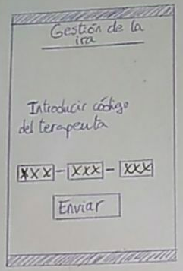
\includegraphics[width=0.8\linewidth, height=7cm]{Imagenes/04DescProblema/mockups/v1/android/02-emparejar.png}
        \caption[Mockup de la 1ª iteración para emparejar dispositivo en la aplicación (opción I)]{Mockup de la 1ª iteración para emparejar dispositivo en la aplicación (opción I)}
        \label{c4:fig:v1:android:emparejar}
    \end{minipage}
    \hfill\vline\hfill
    \begin{minipage}{.45\textwidth}
        \centering
        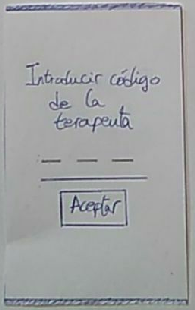
\includegraphics[width=0.8\linewidth, height=7cm]{Imagenes/04DescProblema/mockups/v1/android/02-emparejar-2.png}
        \caption[Mockup de la 1ª iteración para emparejar dispositivo en la aplicación (opción II)]{Mockup de la 1ª iteración para emparejar dispositivo en la aplicación (opción II)}
        \label{c4:fig:v1:android:emparejar2}
    \end{minipage}
\end{figure}

\paragraph{}
En la figura~\ref{c4:fig:v1:android:principal}, aparece la pantalla con el nivel actual de ira del paciente. Si el paciente tiene un nivel de ira elevado (se encuentra inmerso en un episodio de ira) en esta pantalla también aparecen la pauta recomendada y la opción para introducir un comentario (por ejemplo, si decide no seguir la pauta recomendada).

\paragraph{}
La pantalla de la figura~\ref{c4:fig:v1:android:principal2} es una alternativa que une en la misma pantalla la información de la ira y el calibrado de la pulsera. En ella, aparece el nivel de ira y las pautas recomendadas se combinan con la pantalla para sincronizar el dispositivo.

\paragraph{}
En la figura~\ref{c4:fig:v1:android:calibrar} aparece la pantalla para calibrar la pulsera. Hasta que no se ha realizado esta calibración, la aplicación permanece bloqueada puesto que es necesario conocer las constantes vitales del paciente para poder medir la ira del usuario. El paciente debe seleccionar si se va a dormir o si se ha despertado. Una vez sincronizada la pulsera, esta pantalla ya no vuelve a aparecer. La pantalla de la figura~\ref{c4:fig:v1:android:calibrar2} es la segunda opción que se dio para la calibración. La variación reside principalmente en darle al usuario la información de la hora a la que se acostó y se despertó para que así en caso de que haya errores, esta información le ayude a descubrirlos.

\begin{figure}[H]
    \centering
    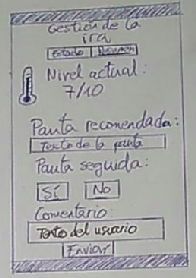
\includegraphics[width=0.36\linewidth, height=7cm]{Imagenes/04DescProblema/mockups/v1/android/01-principal.png}
    \caption[Mockup de la 1ª iteración para ver el estado de ira y la pauta recomendada en la aplicacón]{Mockup de la 1ª iteración para ver el estado de ira y la pauta recomendada en la aplicación}
    \label{c4:fig:v1:android:principal}
\end{figure}


\begin{figure}[H]
    \centering
    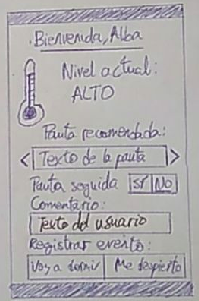
\includegraphics[width=0.4\linewidth, height=8cm]{Imagenes/04DescProblema/mockups/v1/android/01-principal-2.png}
    \caption[Mockup de la 1ª iteración para ver el estado de ira, la pauta recomendada y para calibrar el dispositivo en la aplicación]{Mockup de la 1ª iteración para ver el estado de ira, la pauta recomendada  y para calibrar el dispositivo en la aplicación}
    \label{c4:fig:v1:android:principal2}
\end{figure}

\paragraph{}
Una vez creados los prototipos en papel, se fijó una reunión con la experta en la que se presentaron las distintas alternativas. Las principales conclusiones que se obtuvieron de esta reunión fueron las siguientes:
\begin{itemize}
    \item Las maneras de emparejar la pulsera y el paciente que aparecen en las figuras~\ref{c4:fig:v1:android:calibrar} y~\ref{c4:fig:v1:android:calibrar2} son igualmente apropiadas.
    \item Las dos alternativas para calibrar el dispositivo que se observan en las figuras~\ref{c4:fig:v1:android:calibrar} y~\ref{c4:fig:v1:android:calibrar2} son apropiadas. No ve ninguna razón de peso para elegir una u otra, por lo que finalmente se optó por la alternativa de la figura~\ref{c4:fig:v1:android:calibrar2}, ya que le facilita más información al usuario y le permite rectificar la acción si pulsó accidentalmente alguno de los botones de la pantalla.
    \item El termómetro que aparece en la figura~\ref{c4:fig:v1:android:principal} deberá aparecer en horizontal, estando el menor nivel de ira a la izquierda y el mayor en el otro extremo del termómetro, siguiendo la direccionalidad de la lectura en castellano.

    \begin{figure}[H]
        \centering
        \begin{minipage}{.45\textwidth}
            \centering
            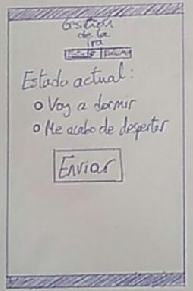
\includegraphics[width=0.8\linewidth, height=7cm]{Imagenes/04DescProblema/mockups/v1/android/03-calibrar.png}
            \caption[Mockup de la 1ª iteración para emparejar dispositivo en la aplicación (opción I)]{Mockup de la 1ª iteración para emparejar dispositivo en la aplicación (opción I)}
            \label{c4:fig:v1:android:calibrar}
        \end{minipage}
        \hfill\vline\hfill
        \begin{minipage}{.45\textwidth}
            \centering
            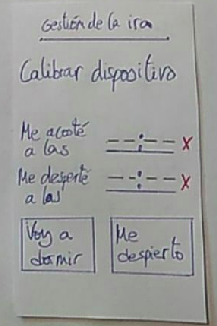
\includegraphics[width=0.8\linewidth, height=7cm]{Imagenes/04DescProblema/mockups/v1/android/03-calibrar-2.png}
            \caption[Mockup de la 1ª iteración para emparejar dispositivo en la aplicación (opción II)]{Mockup de la 1ª iteración para emparejar dispositivo en la aplicación (opción II)}
            \label{c4:fig:v1:android:calibrar2}
        \end{minipage}
    \end{figure}

    \item Para indicar el grado de ira, es mejor hacerlo con palabras (como en la figura~\ref{c4:fig:v1:android:principal2}) que de manera numérica (como en la figura~\ref{c4:fig:v1:android:principal}). Los estados que discreticen el grado de ira que verá el paciente deberán ser reducidos para que el paciente pueda identificar su ordinalidad con facilidad. Así, la solución se limitará a cinco estados: verde, amarillo verdoso, amarillo, naranja y rojo.
    \item Cuando varíe el grado de ira en el termómetro, no solo debe variar cuánto de lleno se encuentra éste, sino también su color. La terapeuta indicó que, tal y como comenta Valdez (\citeyear{valdez1994effects}), existe una relación estrecha entre emociones y colores, por lo que establecer, por ejemplo, que el rojo es el estado de calma y el verde es el estado de mayor percepción de la ira es un cambio significativo respecto a la asociación habitual. En estudios experimentales se ha podido comprobar que los colores de mayor longitud de onda como son el rojo o el amarillo provocan mayor activación que otros de menor longitud de onda como es el verde. A su vez, Jacobs y Sues (\citeyear{jacobs1975effects}) han comprobado en un estudio con los colores rojo, amarillo, verde y azul que existe una mayor asociación del estrés con los colores rojo y amarillo respecto al verde y el azul. Así, a la hora de representar los colores asociados a cada nivel de ira, los colores asociados a estos niveles deberían ser (de menor a mayor nivel de ira): verde, verde-amarillo, amarillo, amarillo-rojo, rojo.
    \item Es importante que el paciente pueda cambiar de pauta si esta no le es útil, tal y como aparece en la figura~\ref{c4:fig:v1:android:principal2}.
    \item El comentario de las pautas que aparece en las figuras~\ref{c4:fig:v1:android:principal} y ~\ref{c4:fig:v1:android:principal2} debe ser opcional y se debe poder añadir usando la voz.
    \item Se deben incluir elementos sonoros que incrementen su volumen en función del nivel de ira del paciente para que este pueda ser consciente de que ha aumentado su nivel de ira.
    \item En la pantalla de la gestión de la ira se debe permitir al paciente seleccionar el tipo de situación que ha generado la ira mediante un seleccionador de causas genéricas que puedan haber ocasionado la situación de ira (por ejemplo, percibir una situación de injusticia).
\end{itemize}

\begin{figure}[H]
    \centering
    \begin{minipage}{.4\textwidth}
        \centering
        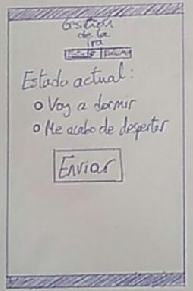
\includegraphics[width=0.8\linewidth, height=7cm]{Imagenes/04DescProblema/mockups/v1/android/03-calibrar.png}
        \caption[Mockup de la 1ª iteración para calibrar el dispositivo en la aplicación (opción I)]{Mockup de la 1ª iteración para calibrar el dispositivo en la aplicación (opción I)}
        \label{c4:fig:v1:android:calibrar}
    \end{minipage}
    \hfill\vline\hfill
    \begin{minipage}{.4\textwidth}
        \centering
        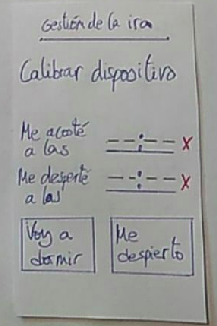
\includegraphics[width=0.8\linewidth, height=7cm]{Imagenes/04DescProblema/mockups/v1/android/03-calibrar-2.png}
        \caption[Mockup de la 1ª iteración para calibrar el dispositivo en la aplicación (opción II)]{Mockup de la 1ª iteración para calibrar el dispositivo en la aplicación (opción II)}
        \label{c4:fig:v1:android:calibrar2}
    \end{minipage}
\end{figure}

\subsubsection{Diseño de la aplicación web del terapeuta}

\paragraph{}
En la figura~\ref{c4:fig:v1:web:iniciarSesion} se muestra la pantalla de inicio de sesión para el terapeuta, mientras que en la figura~\ref{c4:fig:v1:web:registrarPaciente} se muestra la pantalla para registrar a un nuevo paciente.

\begin{figure}[H]
    \centering
    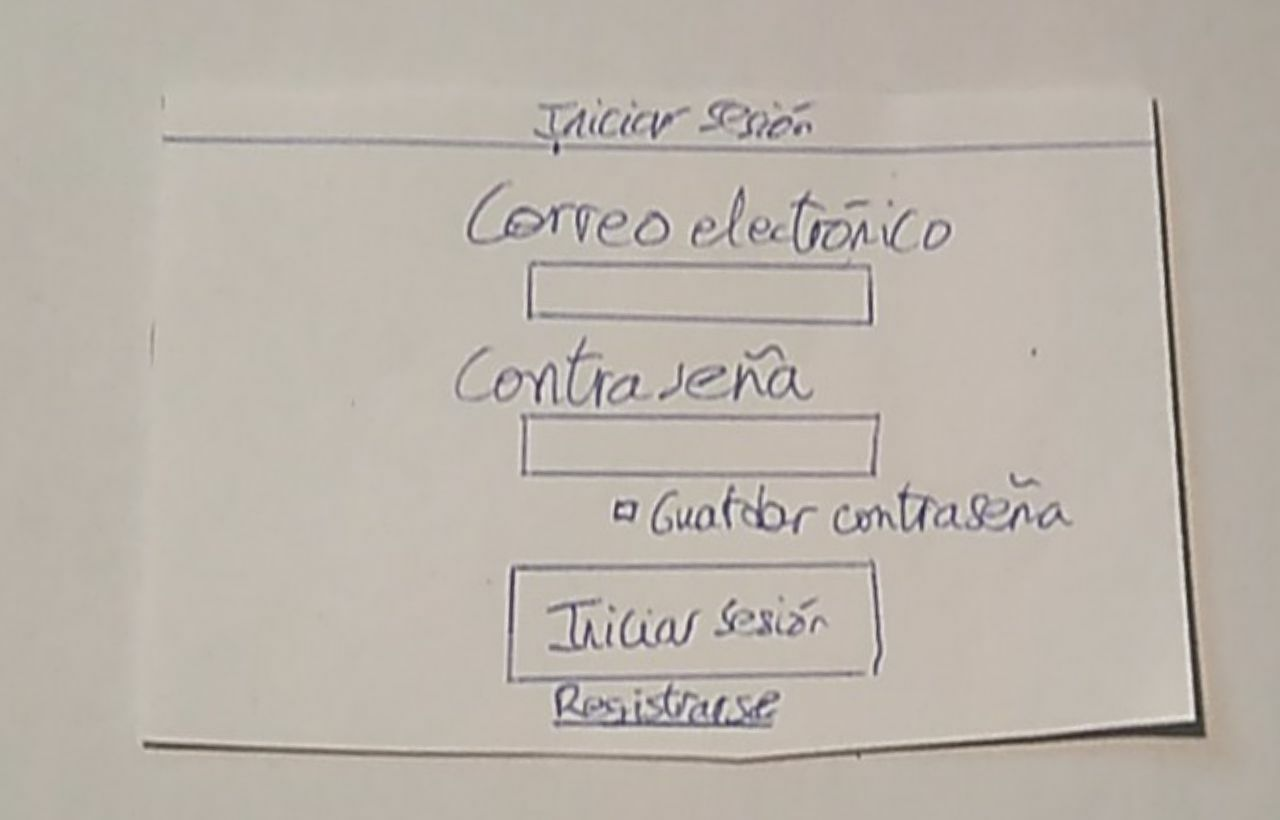
\includegraphics[width=0.7\linewidth, height=8cm]{Imagenes/04DescProblema/mockups/v1/web/01-iniciarSesion.jpg}
    \caption[Mockup de la 1ª iteración para iniciar sesión en la web]{Mockup de la 1ª iteración para iniciar sesión en la web}
    \label{c4:fig:v1:web:iniciarSesion}
\end{figure}

\begin{figure}[H]
    \centering
    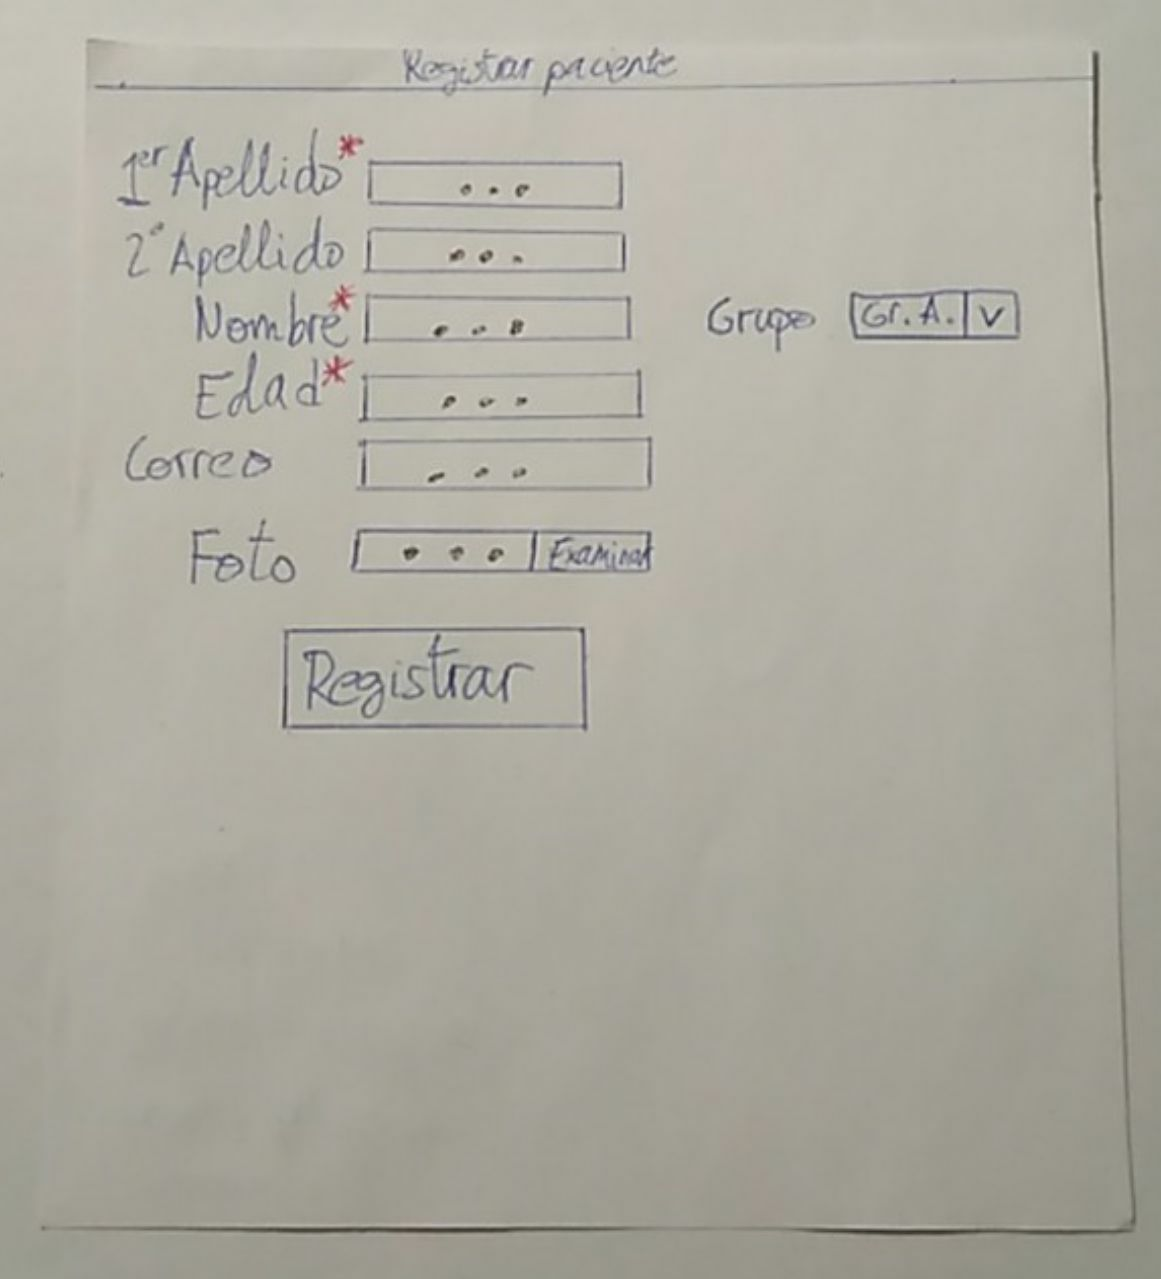
\includegraphics[width=0.7\linewidth, height=8cm]{Imagenes/04DescProblema/mockups/v1/web/02-registrarPaciente.jpg}
    \caption[Mockup de la 1ª iteración para registrar paciente en la web]{Mockup de la 1ª iteración para registrar paciente en la web}
    \label{c4:fig:v1:web:registrarPaciente}
\end{figure}

\paragraph{}
En la figura~\ref{c4:fig:v1:web:modificarGrupo} muestra la pantalla para la creación de grupos con sus pacientes asociados.

\paragraph{}
En las figuras~\ref{c4:fig:v1:web:pautasPaciente} y~\ref{c4:fig:v1:web:pautasPaciente2} se muestran dos alternativas para mostrar las pautas asociadas a cada paciente: una única tabla para todos los niveles de activación en la que se cuenta con una columna con el porcentaje de efectividad general entre los pacientes y una segunda con el texto de la pauta. La primera opción es más visual y cuenta con menos información: no se incluye la columna del porcentaje de éxito de cada pauta y las pautas están divididas en tablas según el nivel de activación asociado.

\begin{figure}[H]
    \centering
    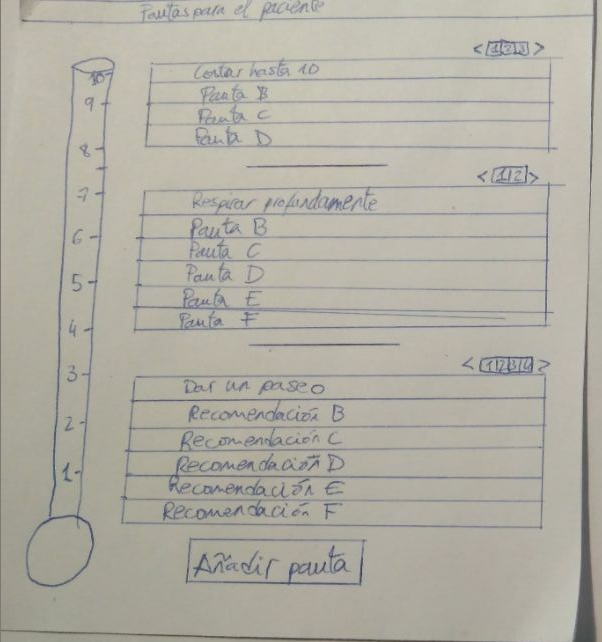
\includegraphics[width=0.7\linewidth, height=8cm]{Imagenes/04DescProblema/mockups/v1/web/04-pautasPaciente.png}
    \caption[Mockup de la 1ª iteración para gestionar pautas en la web (opción I)]{Mockup de la 1ª iteración para gestionar pautas en la web (opción I)}
    \label{c4:fig:v1:web:pautasPaciente}
\end{figure}

\begin{figure}[H]
    \centering
    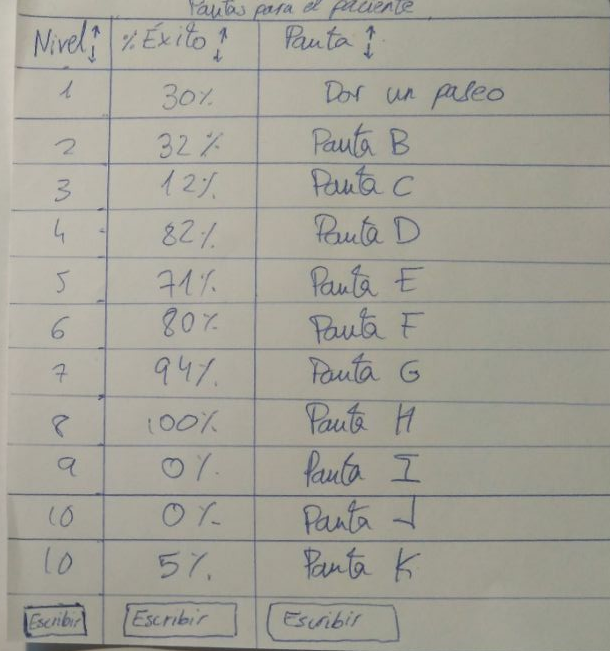
\includegraphics[width=0.7\linewidth, height=8cm]{Imagenes/04DescProblema/mockups/v1/web/04-pautasPaciente-2.png}
    \caption[Mockup de la 1ª iteración para gestionar pautas en la web (opción II)]{Mockup de la 1ª iteración para gestionar pautas en la web (opción II)}
    \label{c4:fig:v1:web:pautasPaciente2}
\end{figure}

\paragraph{}
En la figura~\ref{c4:fig:v1:web:infoPaciente} aparece un elemento genérico para incluir en la cabecera de la pantalla del usuario con información básica sobre este. Al pulsar sobre el botón modificar, se redireccionaría la a pantalla de la figura~\ref{c4:fig:v1:web:gestionarPaciente}.

\begin{figure}[H]
    \centering
    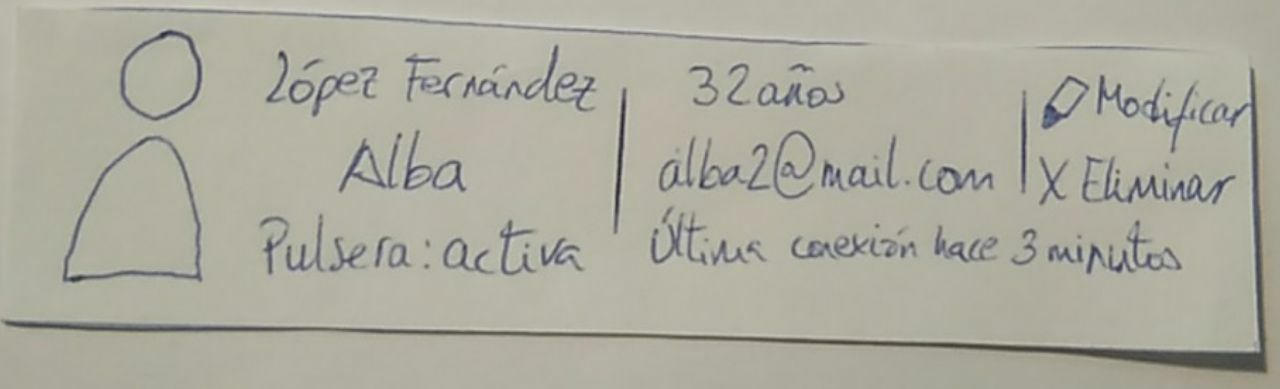
\includegraphics[width=0.7\linewidth, height=5cm]{Imagenes/04DescProblema/mockups/v1/web/07-informacionBasicaPaciente.jpg}
    \caption[Mockup de la 1ª iteración para mostrar la información básica del paciente en la web]{Mockup de la 1ª iteración para mostrar la información básica del paciente en la web}
    \label{c4:fig:v1:web:infoPaciente}
\end{figure}


\paragraph{}
En la figura~\ref{c4:fig:v1:web:gestionarPaciente} aparece la pantalla para modificar el paciente en la que se encuentra la información asociada a las pautas que le han ido apareciendo en la aplicación móvil al paciente. En la parte superior se pueden ver los campos con la información personal del paciente (nombre, apellidos, edad y correo electrónico), el grupo o grupos en los que opcionalmente esté englobado y su foto de perfil. En la parte inferior de la pantalla se puede ver una tabla con las pautas asociadas y la posibilidad de agregar una pauta nueva a ese paciente sin salir de esa pantalla. Si se pulsase sobre el botón cancelar, todos los cambios no guardados se perderían.

\paragraph{}
En las figuras~\ref{c4:fig:v1:web:tablaEpisodios},~\ref{c4:fig:v1:web:tablaEpisodios2} y~\ref{c4:fig:v1:web:tablaEpisodios3} aparecen las tres opciones que se presentaban a la terapeuta para cada paciente en el que se podía ver el resumen de episodios de cada paciente. Las opciones de las figuras~\ref{c4:fig:v1:web:tablaEpisodios} y~\ref{c4:fig:v1:web:tablaEpisodios2} consisten en tablas en las que en una aparece las pautas que se recomendaban y en la figura~\ref{c4:fig:v1:web:tablaEpisodios} se mostraría si la pauta suministrada funcionó o no. La tercera opción sería la de la figura~\ref{c4:fig:v1:web:tablaEpisodios3} en el que se puede ver un histograma con los distintos episodios acaecidos al paciente en cuestión.

\paragraph{}
En la figura~\ref{c4:fig:v1:web:resumenAlertas} aparecen los dos elementos que se utilizarían tanto en la pantalla principal con el resumen de alertas de todos los pacientes como en la pantalla particular de cada paciente. El botón \textit{ver detalles} llevaría a una tabla o gráfica con el resumen de episodios citados.

\begin{figure}[H]
    \centering
    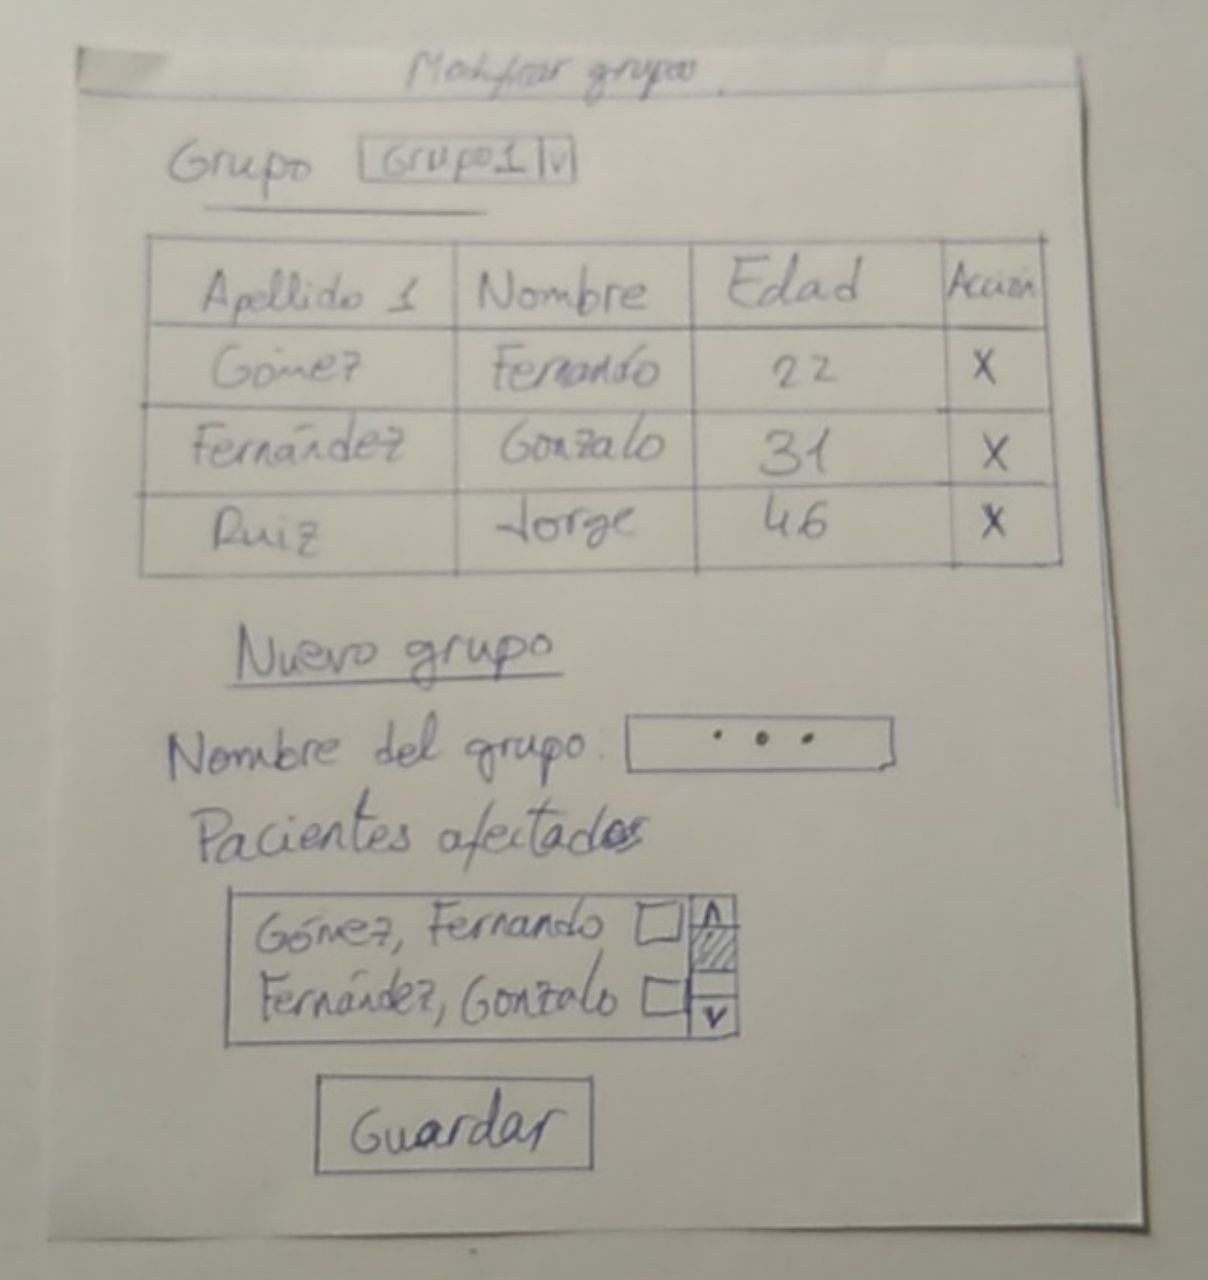
\includegraphics[width=0.8\linewidth, height=8.5cm]{Imagenes/04DescProblema/mockups/v1/web/03-modificarGrupo.jpg}
    \caption[Mockup de la 1ª iteración para gestionar grupos de pacientes en la web]{Mockup de la 1ª iteración para gestionar grupos de pacientes en la web}
    \label{c4:fig:v1:web:modificarGrupo}
\end{figure}

\paragraph{}
En la figura~\ref{c4:fig:v1:web:mostrarEpisodios} aparece el resumen de los episodios de todos los pacientes en el periodo especificado en el segundo elemento de la figura anterior. Así, el elemento más a la izquierda sería un filtro de pacientes similar al que se encuentra en páginas web de compra de artículos en la que se podría filtrar a los mismos en función de la información que se tiene de ellos, así como se podría hacer usando el buscador horizontal que se encuentra en la parte superior de la imagen. Al pulsar sobre cualquiera de estas filas, se abriría la página con el resumen de episodios del paciente seleccionado. La diferencia entre ambas tablas reside principalmente en la utilización del espacio y en que la información provista sea menos o más visual: la opción más a la izquierda, a diferencia de lo que ocurre con la opción de la derecha, no incluiría fotografía y estaría pensada para ocupar menos espacio vertical por registro, lo que permitiría poder representar más registros en el mismo espacio respecto a la segunda opción.

\paragraph{}
En las figuras~\ref{c4:fig:v1:web:resumenAlertas2} y~\ref{c4:fig:v1:web:resumenAlertas3} aparecen dos maneras de representar la suma de las alertas de todos los pacientes del terapeuta para cada nivel en la franja temporal seleccionada (por ejemplo, en la figura~\ref{c4:fig:v1:web:resumenAlertas3} aparece preseleccionado para las últimas 72 horas. La diferencia entre ambos es que en la figura~\ref{c4:fig:v1:web:resumenAlertas2} la información se muestra en un eje cartesiano mientras que en la figura~\ref{c4:fig:v1:web:resumenAlertas3} la información aparece en forma de gráfico de tarta. Estos elementos se incluirían en la página principal de la página web.

\paragraph{}
Una vez creados los prototipos en papel de la aplicación web, nos reunimos con la terapeuta para mostrarselos y buscar el diseño que mejor se ajustase a las necesidades de los usuarios finales. Las principales conclusiones que se obtuvieron de esta reunión fueron las siguientes:

\begin{itemize}
    \item El método de autentificación del terapeuta para iniciar sesión con la tupla correo electrónico y contraseña es apropiado.
    \item A la hora de registrar un paciente, es apropiado poder incluir la foto del paciente para mejorar la visualización. El correo electrónico no es necesario y el grupo al que pertenece cada paciente es prescindible. Para futuras versiones podría ser interesante agrupar a los pacientes y obtener resultados globales de estos grupos pero para esta versión se acaba decidiendo que es mejor centrarse en una solución más sencilla. Por ello, en la figura~\ref{c4:fig:v1:web:registrarPaciente} debe suprimir la selección del grupo.
    \item En cuanto a la forma de representar las pautas de cada paciente (ver figuras~\ref{c4:fig:v1:web:pautasPaciente} y ~\ref{c4:fig:v1:web:pautasPaciente2}), se considera que la solución tiene que ser algo intermedio: se deben dividir las pautas en cinco tablas, que corresponden con los cinco niveles de intensidad de la ira, agrupando las pautas en cada una según su intensidad. Esto es el enfoque de la figura~\ref{c4:fig:v1:web:pautasPaciente}, a lo que habría que añadir columnas adicionales para proporcionar más datos como el porcentaje de éxito de cada pauta, tal y como se puede ver en la figura~\ref{c4:fig:v1:web:pautasPaciente2}.
    \item Se considera apropiado que en el resumen de los episodios de ira figure el tiempo que se mantuvo el paciente en cada uno de los estados, tal y como aparece en el primer elemento de la figura~\ref{c4:fig:v1:web:tablaEpisodios2}.
    \item La información de la pauta recomendada para cada episodio, tal y como aparece en el tercer elemento de la figura~\ref{c4:fig:v1:web:tablaEpisodios2} se considera apropiada, pero es incompleto, ya que para un mismo estado al paciente se le puede haber recomendado más de una pauta, por lo que habría que dividir las celdas correspondientes a las pautas recomendadas para cada intervalo de tiempo en tantas celdas como pautas se hayan recomendado.
    
    \item La representación de las alertas que aparecen en las figuras~\ref{c4:fig:v1:web:resumenAlertas2} y ~\ref{c4:fig:v1:web:resumenAlertas3} son incorrectas, puesto que el número de alertas del paciente debe estar agrupado por episodios, y estos a su vez deben incluir las pautas que se proporcionaron al paciente en cada estado, cuáles fueron descartadas y cuáles no. En la figura~\ref{c4:fig:v1:web:tablaEpisodios3} la representación de episodios en histogramas es correcta pero incompleta, puesto que es necesario que sea una gráfica interactiva que permita poder ampliarla para poder seleccionar y explorar el contenido de estos episodios de manera individualizada.
    
    %\item Las figuras~\ref{c4:fig:v1:web:resumenAlertas} y ~\ref{fig:c4:mockup18} son elementos adicionales que sirven para decorar las pantallas que se generaron. La figura~\ref{c4:fig:v1:web:resumenAlertas} se considera apropiada mientras que el primer elemento de la figura~\ref{fig:c4:mockup18} se considera que no aporta información útil para la terapeuta.
    
    \item Los filtros de la figura~\ref{c4:fig:v1:web:mostrarEpisodios} se consideran apropiados. Sin embargo, la información sobre el número de alertas de cada una de las intensidades de la ira de cada paciente no es relevante, ya que esta información sin estar agrupada en episodios y desglosada por fechas no aporta información util al terapeuta.
\end{itemize}



\begin{figure}[H]
    \centering
    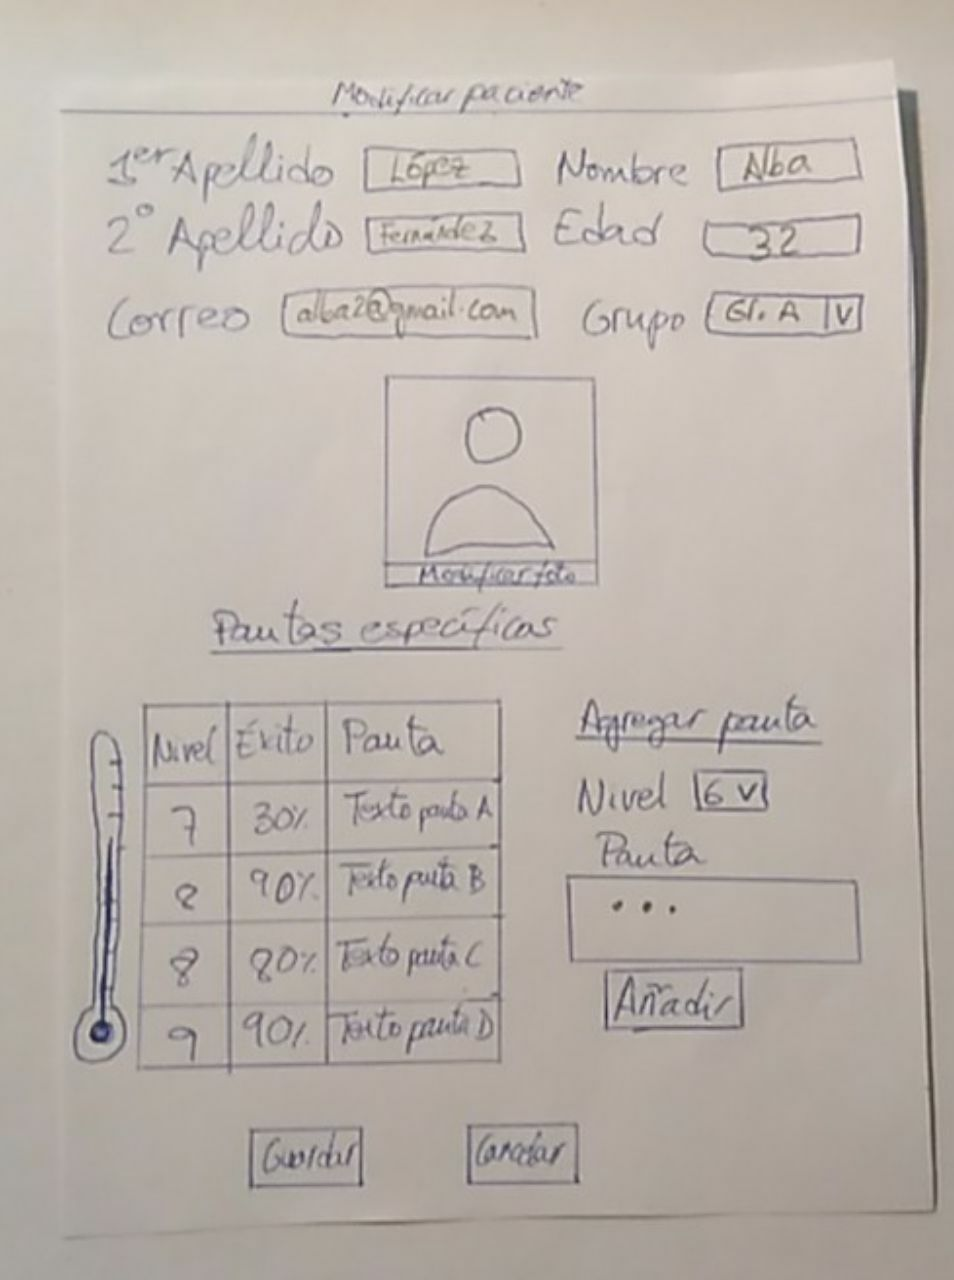
\includegraphics[width=0.7\linewidth, height=8cm]{Imagenes/04DescProblema/mockups/v1/web/05-modificarPaciente.jpg}
    \caption[Mockup de la 1ª iteración para gestionar un paciente en la web]{Mockup de la 1ª iteración para gestionar un paciente en la web}
    \label{c4:fig:v1:web:gestionarPaciente}
\end{figure}

\begin{figure}[H]
    \centering
    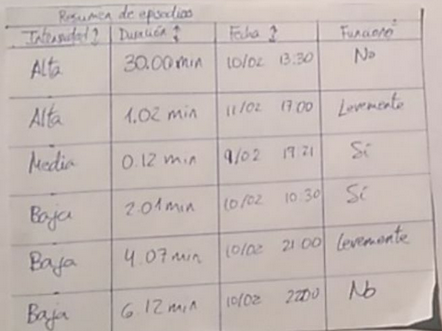
\includegraphics[width=0.7\linewidth, height=8cm]{Imagenes/04DescProblema/mockups/v1/web/06-resumenEpisodios.png}
    \caption[Mockup de la 1ª iteración para mostrar los episodios de un paciente en la web (opción I)]{Mockup de la 1ª iteración para mostrar los episodios de un paciente en la web (opción I)}
    \label{c4:fig:v1:web:tablaEpisodios}
\end{figure}

\begin{figure}[H]
    \centering
    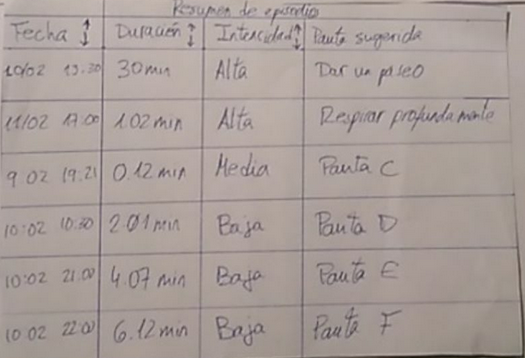
\includegraphics[width=0.7\linewidth, height=8cm]{Imagenes/04DescProblema/mockups/v1/web/06-resumenEpisodios-2.png}
    \caption[Mockup de la 1ª iteración para mostrar los episodios de un paciente en la web (opción II)]{Mockup de la 1ª iteración para mostrar los episodios de un paciente en la web (opción II)}
    \label{c4:fig:v1:web:tablaEpisodios2}
\end{figure}

\begin{figure}[H]
    \centering
    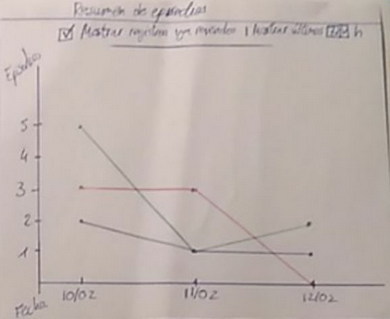
\includegraphics[width=0.7\linewidth, height=8cm]{Imagenes/04DescProblema/mockups/v1/web/06-resumenEpisodios-3.png}
    \caption[Mockup de la 1ª iteración para mostrar los episodios de un paciente en la web (opción III)]{Mockup de la 1ª iteración para mostrar los episodios de un paciente en la web (opción III)}
    \label{c4:fig:v1:web:tablaEpisodios3}
\end{figure}


\begin{figure}[H]
    \centering
    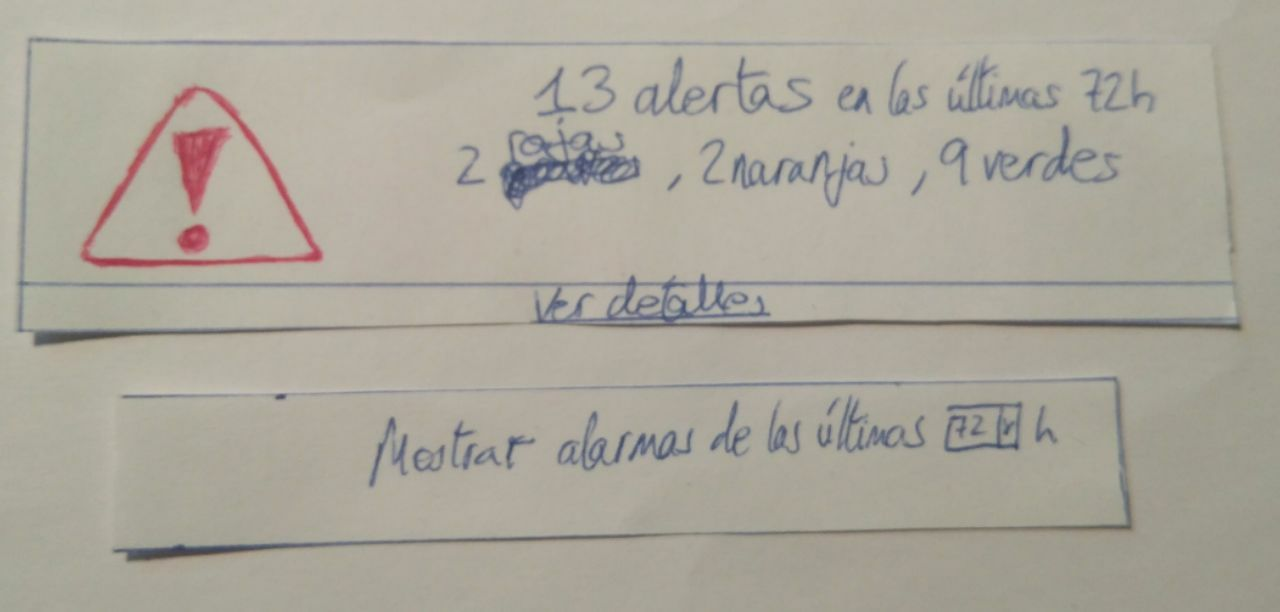
\includegraphics[width=0.7\linewidth, height=8cm]{Imagenes/04DescProblema/mockups/v1/web/08-alertas.jpg}
    \caption[Mockup de la 1ª iteración para mostrar alertas de los episodios de ira en la web]{Mockup de la 1ª iteración para mostrar alertas de los episodios de ira en la web}
    \label{c4:fig:v1:web:resumenAlertas}
\end{figure}

\begin{figure}[H]
    \centering
    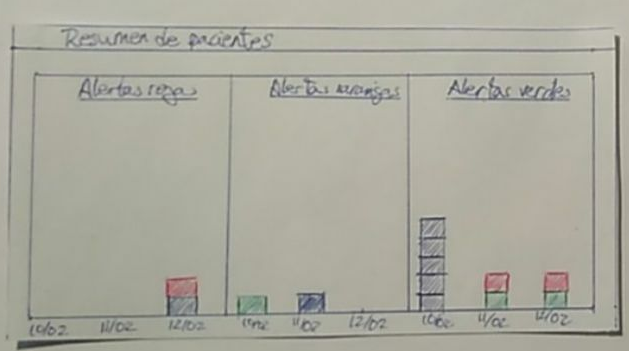
\includegraphics[width=0.7\linewidth, height=8cm]{Imagenes/04DescProblema/mockups/v1/web/08-alertas-2.png}
    \caption[Mockup de la 1ª iteración para mostrar el resumen de alertas de los pacientes en la web (opción I)]{Mockup de la 1ª iteración para mostrar el resumen de alertas de los pacientes en la web (opción I)}
    \label{c4:fig:v1:web:resumenAlertas2}
\end{figure}

\begin{figure}[H]
    \centering
    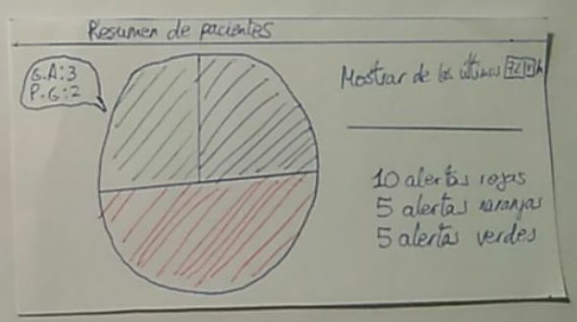
\includegraphics[width=0.7\linewidth, height=8cm]{Imagenes/04DescProblema/mockups/v1/web/08-alertas-3.png}
    \caption[Mockup de la 1ª iteración para mostrar el resumen de alertas de los pacientes en la web (opción II)]{Mockup de la 1ª iteración para mostrar el resumen de alertas de los pacientes en la web (opción II)}
    \label{c4:fig:v1:web:resumenAlertas3}
\end{figure}

\begin{figure}[H]
    \centering
    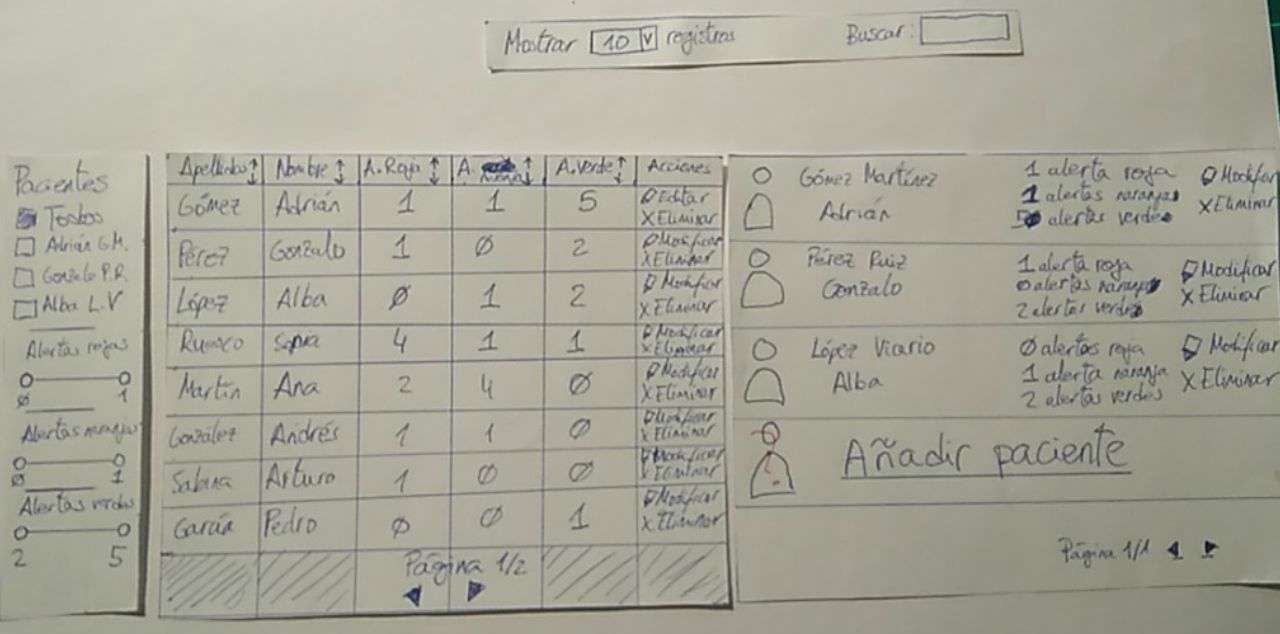
\includegraphics[width=0.8\linewidth, height=7cm]{Imagenes/04DescProblema/mockups/v1/web/09-mostrarEpisodios.jpg}
    \caption[Mockup para mostrar los filtros y las dos opciones para mostrar la tabla de pacientes]{Mockup para mostrar los filtros y las dos opciones para mostrar la tabla de pacientes}
    \label{c4:fig:v1:web:mostrarEpisodios}
\end{figure}

\subsection{Segunda iteración}

\paragraph{}
Para esta segunda iteración, se usaron prototipos de alta fidelidad con Android para crear el segundo prototipo de la aplicación móvil del paciente y HTML para crear el segundo prototipo de la aplicación web del terapeuta para que estos fueran lo más similares posibles al resultado final de la aplicación. Esto se debe a que, tras la primera iteración, se pudieron extraer los suficientes requisitos como para poder avanzar en detalles más concretos de la aplicación final.

\subsubsection{Diseño de la aplicación móvil de los pacientes}


\begin{figure}[H]
    \centering
    \begin{minipage}{.45\textwidth}
        \centering
        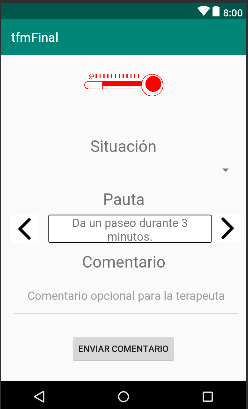
\includegraphics[width=0.8\linewidth, height=7cm]{Imagenes/04DescProblema/mockups/v2/android/01-principal.png}
        \caption[Mockup de la 2ª iteración para la pantalla principal de la aplicación]{Mockup de la 2ª iteración para la pantalla principal de la aplicación}
        \label{c4:fig:v2:android:principal}
    \end{minipage}
\end{figure}

\begin{figure}[H]
    \centering
    \begin{minipage}{.45\textwidth}
        \centering
        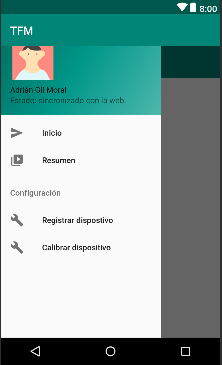
\includegraphics[width=0.8\linewidth, height=7cm]{Imagenes/04DescProblema/mockups/v2/android/02-menu.png}
        \caption[Mockup de la 2ª iteración para el menú de la aplicación]{Mockup de la 2ª iteración para el menú de la aplicación}
        \label{c4:fig:v2:android:menu}
    \end{minipage}
\end{figure}

\begin{figure}[H]
    \centering
    \begin{minipage}{.45\textwidth}
        \centering
        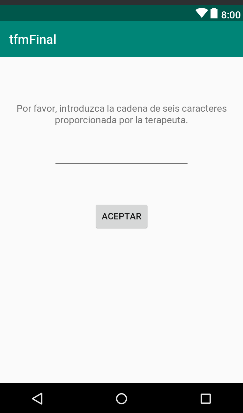
\includegraphics[width=0.9\linewidth, height=8cm]{Imagenes/04DescProblema/mockups/v2/android/03-emparejar.png}
        \caption[Mockup de la 2ª iteración para emparejar el dispositivo en la aplicación]{Mockup de la 2ª iteración para emparejar el dispositivo en la aplicación}
        \label{c4:fig:v2:android:emparejar}
    \end{minipage}
\end{figure}

\begin{figure}[H]
    \centering
    \begin{minipage}{.45\textwidth}
        \centering
        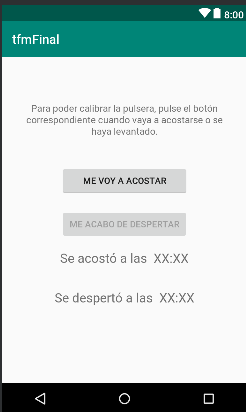
\includegraphics[width=0.9\linewidth, height=8cm]{Imagenes/04DescProblema/mockups/v2/android/04-calibrar.png}
        \caption[Mockup de la 2ª iteración para calibrar el dispositivo en la aplicación]{Mockup de la 2ª iteración para calibrar el dispositivo en la aplicación}
        \label{c4:fig:v2:android:calibrar}
    \end{minipage}
\end{figure}

\begin{figure}[H]
    \centering
    \begin{minipage}{.45\textwidth}
        \centering
        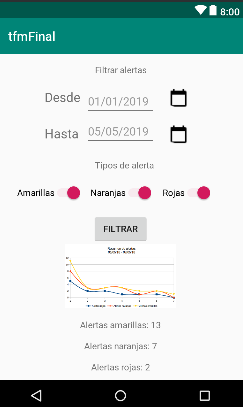
\includegraphics[width=0.8\linewidth, height=7cm]{Imagenes/04DescProblema/mockups/v2/android/05-resumenEpisodios.png}
        \caption[Mockup de la 2ª iteración para mostrar el resumen de episodios en la aplicación]{Mockup de la 2ª iteración para mostrar el resumen de episodios en la aplicación}
        \label{c4:fig:v2:android:episodios}
    \end{minipage}
\end{figure}

\paragraph{}
Las pantallas de esta segunda fase de diseño de la aplicación móvil son las siguientes:

\begin{itemize}
    \item En la figura~\ref{c4:fig:v2:android:menu} se puede ver el menú de la aplicación. En lugar de tener un menú horizontal que quite espacio para el resto de pantallas, este menú se desplegará como se hace en aplicaciones como Telegram o Whatsapp mediante el pulsado en un bocadillo a la izquierda de la barra horizontal superior o mediante el desplazamiento de la pantalla de izquierda a derecha. Este menú se habilitaría después de haber emparejado el dispositivo en la pantalla de la figura~\ref{c4:fig:v2:android:emparejar}. En la parte superior del menú se encontraría la información personal del paciente que la terapeuta rellenó en el registro del paciente en la aplicación web. En la parte inferior se encuentran los cuatro elementos del menú: el botón de inicio que redireccionaría a la pantalla~\ref{c4:fig:v2:android:principal}, el botón para ver el resumen de episodios, que redireccionaría a la pantalla ~\ref{c4:fig:v2:android:episodios}, el botón para registrar el dispositivo, que redireccionaría a la pantalla ~\ref{c4:fig:v2:android:emparejar} y el botón para calibrar el dispositivo, que redireccionaría a la pantalla ~\ref{c4:fig:v2:android:calibrar}.
    \item En la figura~\ref{c4:fig:v2:android:emparejar} aparece la pantalla para introducir el código para sincronizar la pulsera y el móvil con el paciente. Una vez se haya emparejado el dispositivo, en esta pantalla aparecerá en formato de texto y de manera no editable la fecha y la hora en la que se produjo el emparejamiento.
    \item En la figura~\ref{c4:fig:v2:android:calibrar} podemos ver la pantalla para calbirar el dispositivo durante su primer uso. Cuando el paciente se acueste, deberá indicarlo en la aplicación pulsando sobre el botón "me voy a acostar". Este botón cambiará su literal a "cancelar", el literal "Se acostó a las XX:XX" será reemplazado por la hora en la que el paciente indicó que se acostó y el botón "me voy a acostar dejará de estar inhabilitado. Si el paciente pulsó este botón por accidente, al pulsar sobre cancelar se volverá al estado inicial. Cuando el paciente pulse sobre el botón "me acabo de desperar", se almacenará en la aplicación la hora a la que se despertó y la hora a la que se acostó el paciente. Tras realizar esta operación, los elementos de esta pantalla serán sustituidos por unos literales no editables en los que se indiquen la fecha y hora en la que se produjo esta calibración.
    \item En la figura ~\ref{c4:fig:v2:android:principal} se encuentra la pantalla principal de la aplicación con la información sobre el estado de la ira del paciente. En esta pantalla, en el caso de que el paciente esté inmerso en un episodio de ira, aparecerá una pauta recomendada para intentar disminuir el nivel de ira con el nivel de ira representado mediante un termómetro horizontal. El paciente usando las flechas podrá cambiar de pauta y tendrá la opción de enviar comentarios sobre la pauta o el episodio en cuestión.
    
    \item En la figura~\ref{c4:fig:v2:android:episodios} se muestra la pantalla de resumen de la evolución de los episodios seguida por el paciente en formato histograma.
\end{itemize}

\paragraph{}
Al revisar este nuevo diseño con la terapeuta, se obtuvieron las siguientes conclusiones:

\begin{itemize}
    \item Las pantallas que se muestran se ajustan bastante a lo esperado por parte de la terapeuta, pero hay que introducir el concepto de episodio. La terapeuta define un episodio como un conjunto cronológicamente ordenado de alertas que empieza en el estado de reposo y acaba en el estado de reposo. Esa debe ser la unidad mínima con la que el terapeuta debe trabajar y no usar la alerta como unidad mínima.
    \item El termómetro con el nivel de ira de la figura~\ref{c4:fig:v2:android:principal} debe ir al revés: el elemento de mayor grosor tiene que ir a la izquierda (que representará el menor nivel de ira).
    \item Se debe incluir un \textit{widget}\footnote{Un \textit{widget} es una pequeña aplicación para el móvil que permite al usuario visualizar en la pantalla de inicio información dinámica de una aplicación sin que sea necesario que el usuario interactúe con la aplicación. Un ejemplo sería un \textit{widget} para mostrar el nivel de batería en el móvil.} en la aplicación en el que aparezca un pequeño termómetro con el nivel de ira del paciente en ese momento para que el paciente pueda ver su estado actual de la ira sin necesidad de abrir la aplicación.
    \item Se deben incluir mensajes de alertas motivacionales tipo \textit{toast}\footnote{Un \textit{toast} es un mensaje flotante rectangular que se puede visualizar en el móvil sin tener abierta la aplicación que lo ha emitido.} como refuerzo positivo para el paciente cuando se detecte una disminución continuada de sus episodios de ira.
    \item A la hora de interpretar la actividad fisiológica del paciente, es necesario discernir entre episodios de ira y episodios provocados por actividades que puedan generar mayor activación que no impliquen episodios de ira (como al realizar ejercicio físico o al mantener relaciones sexuales).
    \item En esta iteración se ha echado en falta poder ver cómo quedaría la pantalla principal de la aplicación móvil con el estado de la ira del paciente ( figura~\ref{c4:fig:v2:android:principal}) cuando el paciente no está experimentando un episodio de ira.
    \item En la pantalla principal (figura~\ref{c4:fig:v2:android:principal}) es necesario añadir que el paciente pueda seleccionar entre una lista de opciones la causa principal que ha generado el episodio de ira que está experimentando.
    \item Una vez que se ha sugerido una pauta al paciente, pasado un tiempo, habrá que preguntar al usuario si ha seguido la pauta que se le ha recomendado. Si responde afirmativamente y el paciente no se encuentra en estado de reposo, se le mostrarán más pautas acordes a su nivel actual de ira. Si responde negativamente, se preguntará al paciente por qué no ha seguido la pauta y, a continuación, se le mostrará una nueva pauta.
\end{itemize}

\subsubsection{Diseño de la aplicación web del terapeuta}

\begin{figure}[H]
    \centering
    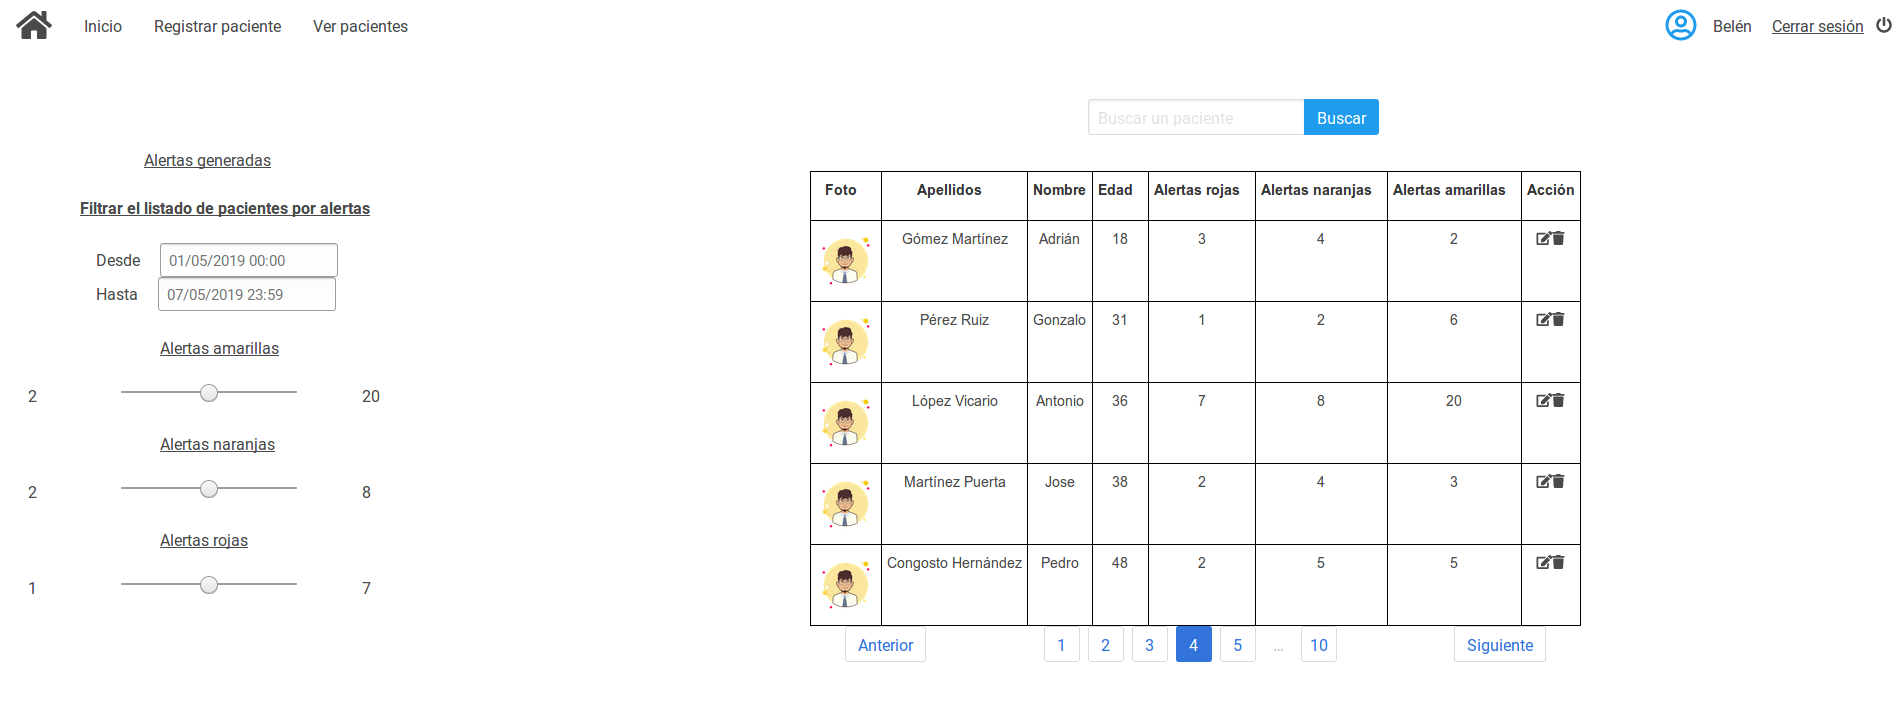
\includegraphics[width=0.8\linewidth, height=7cm]{Imagenes/04DescProblema/mockups/v2/web/01-principal.png}
    \caption[Mockup de la 2ª iteración de la pantalla principal de la web]{Mockup de la 2ª iteración de la pantalla principal de la web}
    \label{c4:fig:v2:web:principal}
\end{figure}

\begin{figure}[H]
    \centering
    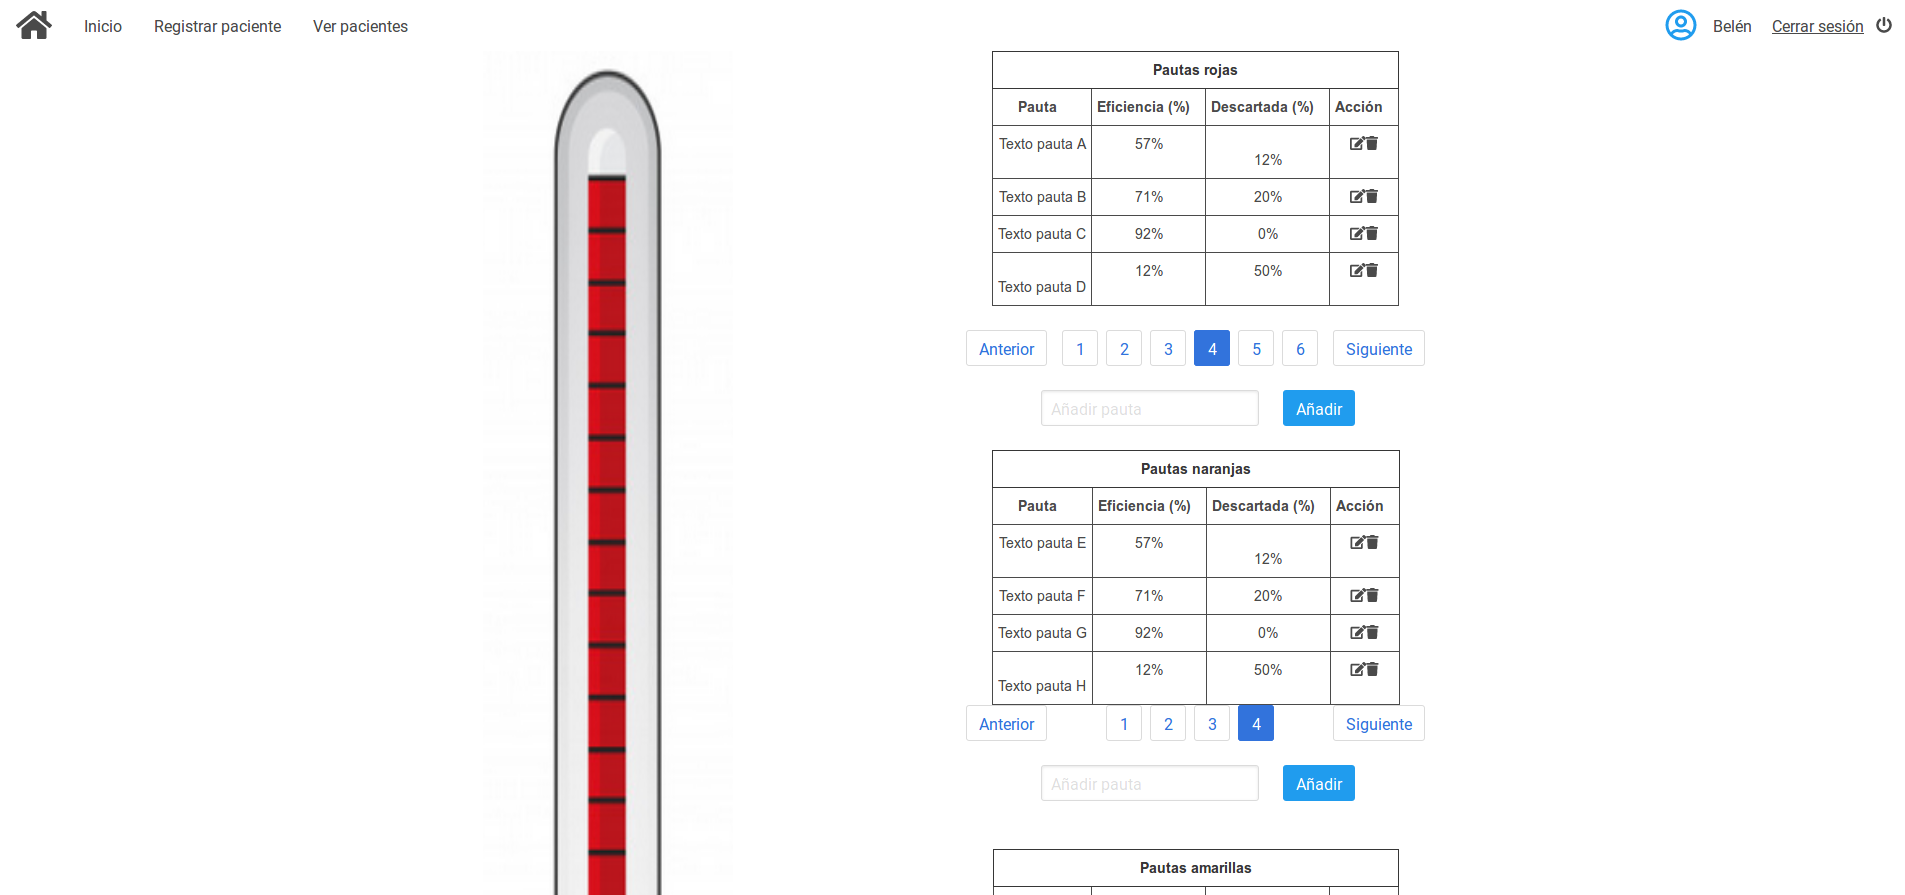
\includegraphics[width=0.8\linewidth, height=7cm]{Imagenes/04DescProblema/mockups/v2/web/02-pautas.png}
    \caption[Mockup de la 2ª iteración de la pantalla de pautas de la web]{Mockup de la 2ª iteración de la pantalla de pautas de la web}
    \label{c4:fig:v2:web:pautas}
\end{figure}

\begin{figure}[H]
    \centering
    \begin{minipage}{.45\textwidth}
        \centering
        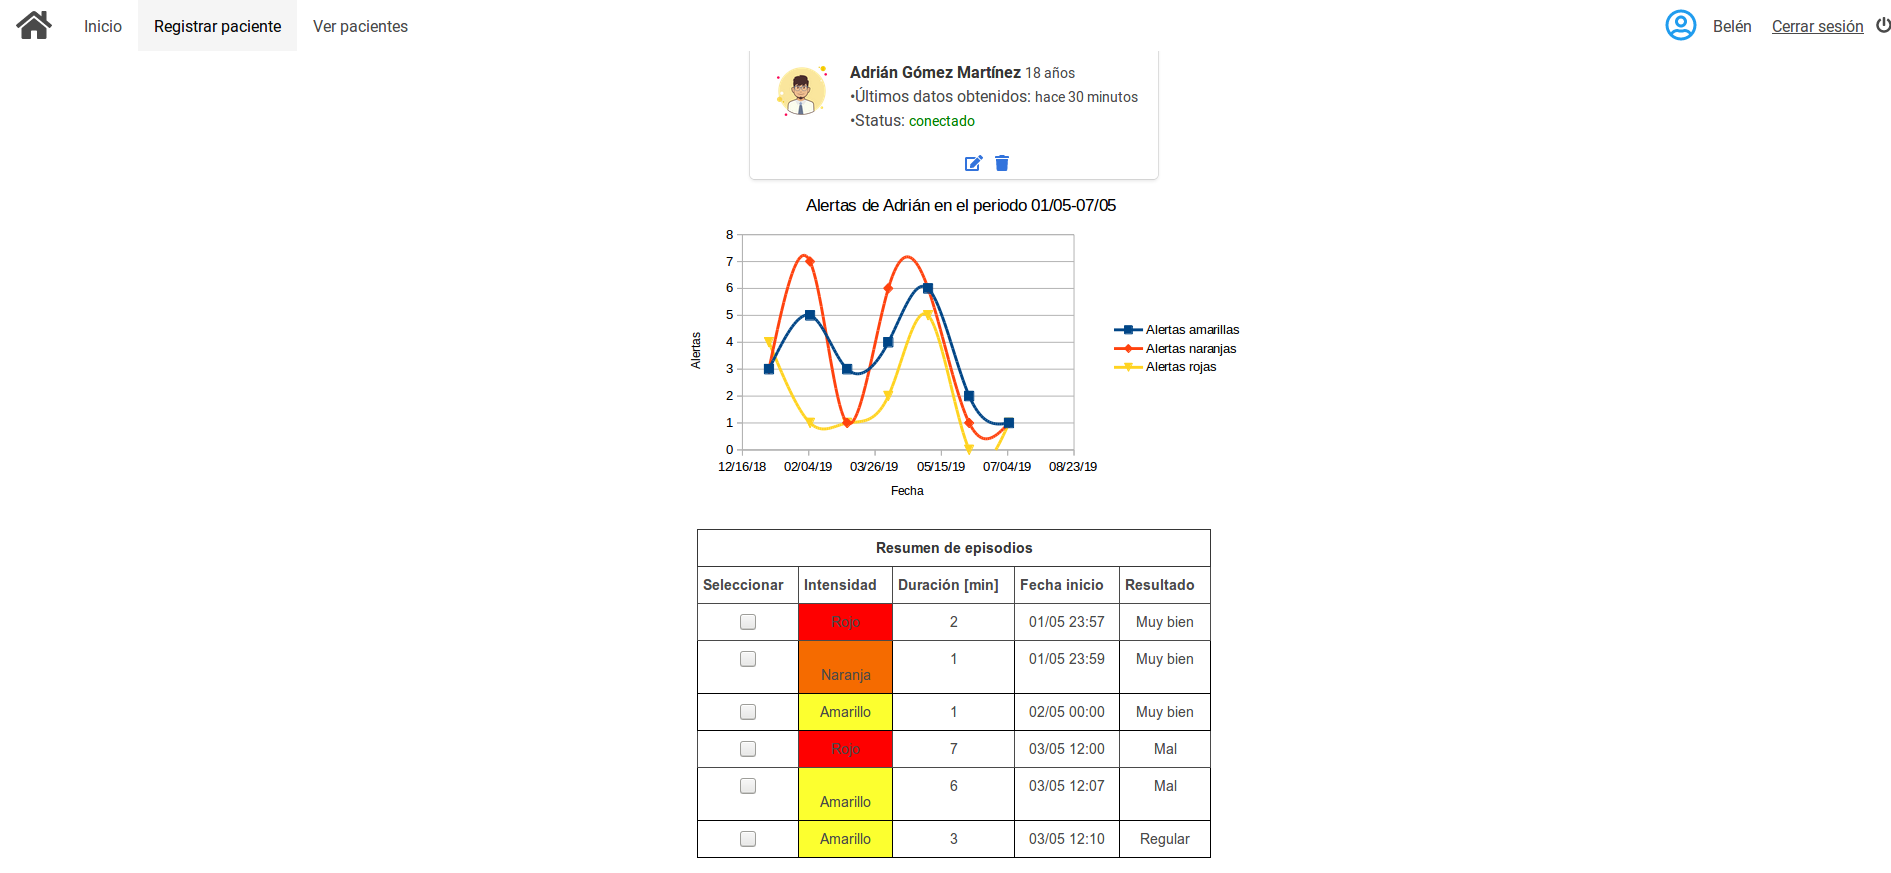
\includegraphics[width=0.8\linewidth, height=7cm]{Imagenes/04DescProblema/mockups/v2/web/03-resumenEpisodios.png}
        \caption[Mockup de la 2ª iteración de la pantalla de resumen de episodios de la web (parte I)]{Mockup de la 2ª iteración de la pantalla de resumen de episodios de la web (parte I)}
        \label{c4:fig:v2:web:episodios1}
    \end{minipage}
\end{figure}

\begin{figure}[H]
    \centering
    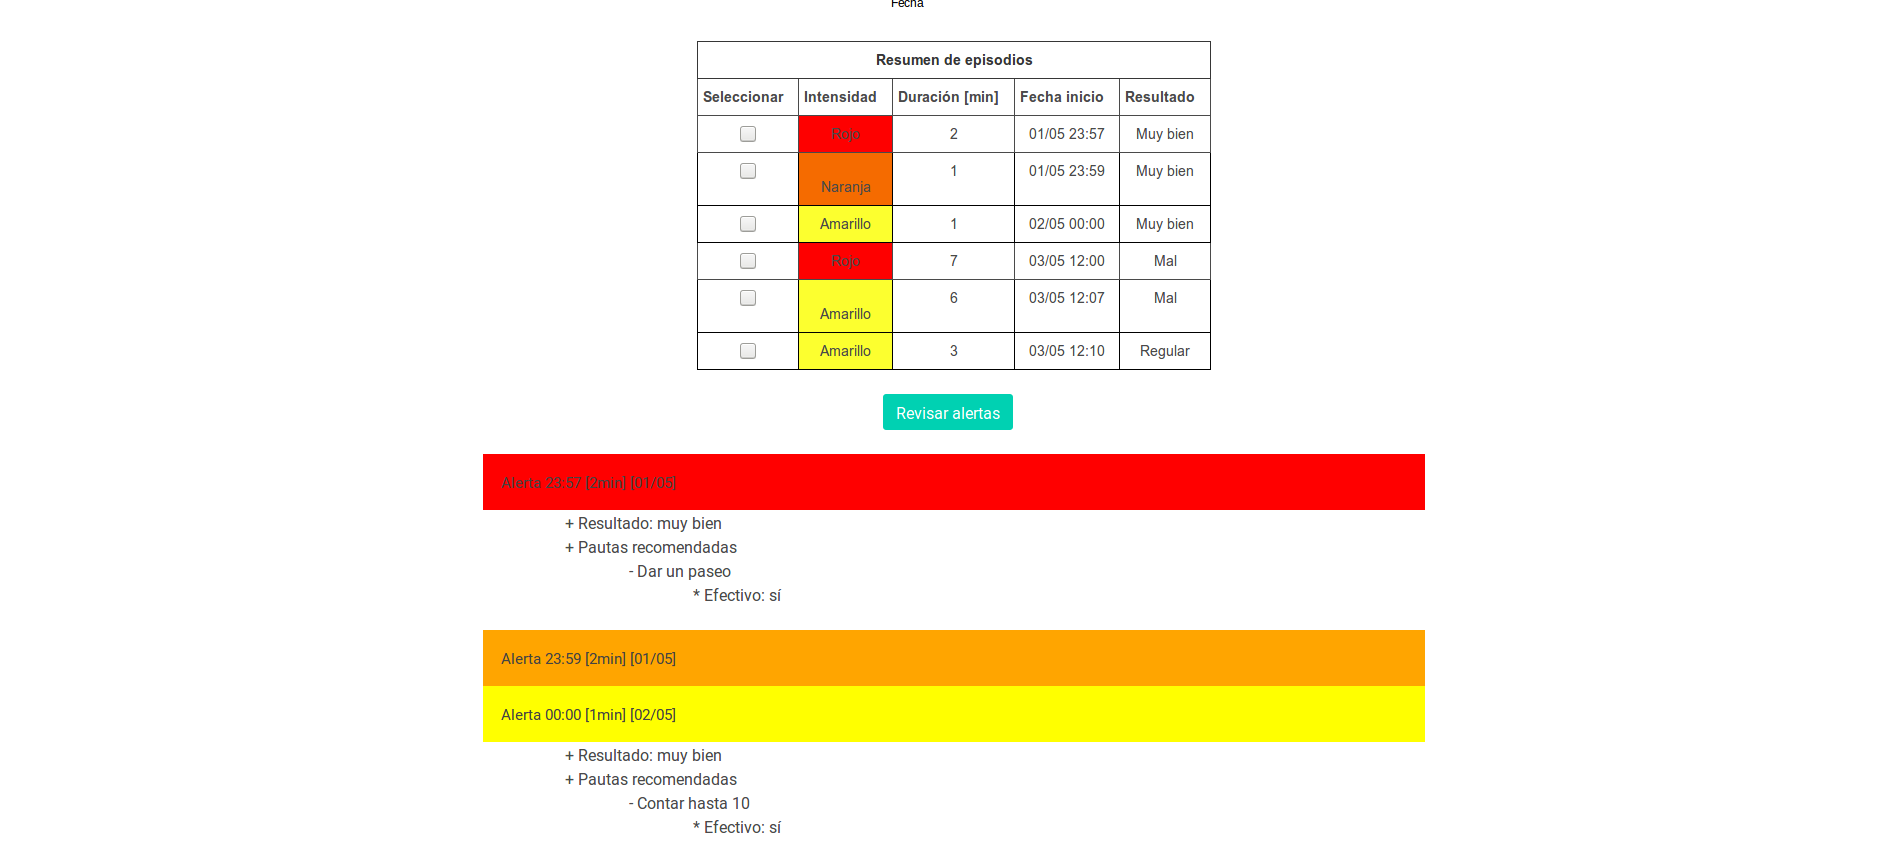
\includegraphics[width=0.8\linewidth, height=7cm]{Imagenes/04DescProblema/mockups/v2/web/03-resumenEpisodios-2.png}
    \caption[Mockup de la 2ª iteración de la pantalla de resumen de episodios de la web (parte II)]{Mockup de la 2ª iteración de la pantalla de resumen de episodios de la web (parte II)}
    \label{c4:fig:v2:web:episodios2}
\end{figure}

\paragraph{}
En este caso, se diseñaron exclusivamente las pantallas que pudieran ser fruto de mayor controversia, puesto que la interfaz de estas funcionalidades ya quedó cerrada en la iteración anterior. Las pantallas de la web que no aparecen en esta iteración por este motivo son las correspdientes a las siguientes funcionalidades: inicio de sesión, registrar/modificar paciente, registrar/modificar pauta y registrar/modificar grupo de pautas.

\paragraph{}
En la figura~\ref{c4:fig:v2:web:principal} podemos ver la pantalla que muestra todos los pacientes que tiene asociados el terapeuta. De cada paciente se muestra la foto, el nombre y apellidos, la edad y el número de alertas de cada tipo. Cada paciente podrá ser borrado o modificado usando los iconos correspondientes de la columna acción. El listado se podrá filtrar por fechas o por el número de alertas.

\paragraph{}
Si se pulsa sobre alguno de los pacientes de la pantalla anterior, se mostrará su información ampliada. Para mostrar esta información, se creó la pantalla de las figuras~\ref{c4:fig:v2:web:episodios1} y~\ref{c4:fig:v2:web:episodios2} (es la misma pantalla cortada en dos imágenes). En la figura~\ref{c4:fig:v2:web:episodios1} se muestra la información básica del paciente, un histograma con el nivel de alertas de cada tipo para un periodo de tiempo de una semana y una tabla con el resumen de los episodios que se han producido en ese periodo de tiempo. En esta tabla, al clicar sobre los checkboxes de la columna "seleccionar" y posteriormente pulsar en el botón "revisar alertas" que aparece en la figura~\ref{c4:fig:v2:web:episodios2}, se mostrarán los elementos que aparecen debajo de este botón. Estos elementos son el desglose de las alertas de los episodios seleccionados, incluyendo las pautas recomendadas y la utilidad de las mismas representadas de manera binaria (si ha sido util o no).

\paragraph{}
En la figura ~\ref{c4:fig:v2:web:pautas} se muestra la pantalla que permite al terapeuta ver las distintas pautas que ha creado. Estas pautas están agrupadas por el nivel de ira del paciente en el que podrían aparecerle al paciente. La tabla tiene cuatro columnas. La primera columna incluye el texto de la pauta que le aparecería al paciente; la segunda columna incluye la eficiencia que esa pauta ha tenido a la hora de reducir el nivel de ira entre todos los pacientes del terapeuta; la tercera columna incluye el porcentaje de veces que dicha pauta ha sido descartada y la cuarta columna incluye las acciones que se pueden realizar sobre dicha pauta: editar o borrar. Al pulsar sobre el botón editar, el campo con el texto de la pauta se podría editar. Por último, si se quiere añadir una pauta, debajo de los marcadores de páginas de pautas de cada nivel de ira se encuentre una entrada de texto en la que se podría incluir el texto de una nueva pauta que se crearía tras clicar sobre el botón "añadir".

\paragraph{}
Tras la reunión con la terapeuta, los puntos que se sacaron en claro fueron los siguientes:

\begin{itemize}
    \item El terapeuta trabaja con los pacientes al nivel de episodios, no de alertas, por lo que tanto la gráfica como el desglose de episodios que aparecen en las figuras~\ref{c4:fig:v2:web:episodios1} y~\ref{c4:fig:v2:web:episodios1} son incorrectas. Es necesario agrupar dichas alertas en episodios, tal y como se ve en la tabla de la figura~\ref{c4:fig:v2:web:episodios1}. Al realizar dicho desglose en el elemento que hay debajo del botón "revisar alertas" de la figura~\ref{c4:fig:v2:web:episodios1}, no debe aparecer el concepto de alerta sino que se tiene que agrupar la información por lapsos de tiempo. Por ejemplo, si en el episodio que se ha seleccionado ha estado 30 segundos en el estado rojo y se determina que el lapso de tiempo por el que se va a agrupar la información es de diez segundos, no tiene que aparecer una única fila para esos treinta segundos de estado, sino tres filas para esos tres lapsos de diez segundos. Esto supone que se va a proporcionar al usuario información más detallada de lo que ha sucedido en ese periodo de tiempo.
    
    \item La gráfica de la figura~\ref{c4:fig:v2:web:episodios1} debe ser interactiva. Se insiste en emular el diseño de los desfibriladores. En concreto, se menciona que se pueda seleccionar una franja temporal en la propia gráfica y que el acordeón que hay en la parte inferior de la figura~\ref{c4:fig:v2:web:episodios2}, se actualice para incluir la información detallada de los episodios contenidos en dicha franja temporal.
    
    \item La pantalla de la figura~\ref{c4:fig:v2:web:pautas} para la gestión de las pautas es correcta.
    \item Se echa en falta una pantalla en la que se indique cómo se vincularían las pautas a cada paciente. A su vez, es necesario poder agrupar pautas de alguna manera para que, cuando haya que vincular las pautas para un nuevo paciente con una sintomatología similar a la de pacientes anteriores, ese agrupamiento pueda servir como guía de las pautas que le pueden ser útiles al nuevo paciente.
\end{itemize}

\subsection{Tercera iteración}
\paragraph{}
En esta iteracción, las pantallas ya no eran elementos estáticos que se mostraban a la experta sino que incluían la parte de programación necesaria del backend y de transiciones entre pantallas para poder ver la manera en la que se gestionan los datos. Las herramientas que se usaron para hacer los mockups de la web y de Android, igual que en la iteración anterior, son las que se utilizaron para la implementación final. Adicionalmente, en el caso de los mockups de la web, estos se hicieron usando el \textit{framework} de estilos CSS Bulma \citep{responsivelearning}, utilizando macros genéricos entre las pantallas para estandarizar el formato entre ellas.

\paragraph{}
A diferencia de lo que ocurría en la segunda iteración, se han definido todas las pantallas, incluidas las que estaban cerradas desde la primera versión, para que así se pudiese valorar el mockup en su conjunto (incluyendo transiciones entre pantallas) en lugar de hacerlo con separaciones bruscas entre las valoraciones de cada pantalla.

\subsubsection{Diseño de la aplicación móvil de los pacientes}
\paragraph{}
\paragraph{}
Las pantallas de esta segunda fase de diseño de la aplicación móvil son las siguientes:

\begin{itemize}
    \item En la pantalla de la figura~\ref{c4:fig:v3:android:01IndexNotCalibrated} aparece la pantalla principal cuando se detecta que el usuario no ha registrado y calibrado el dispositivo. al pulsar sobre el botón "registrar el dispositivo" se cargaría la pantalla de la figura~\ref{c4:fig:v3:android:04RegisterDevice}, mientras que al pulsar el botón "calibrar dispositivo" se cargaría la pantalla de la figura~\ref{c4:fig:v3:android:05CalibrateDevice}. En la parte inferior de la pantalla, aparece un indicador del número de pasos que se han realizado para poder utilizar la aplicación. En este caso, como no se ha registrado ni calibrado el dispositivo, aparece el literal "0/2". El botón para calibrar el dispositivo permanece bloqueado hasta que se registre el dispositivo ya que es necesario realizar primero este paso. Por otro lado, como se verá también en otras pantallas, una vez una pantalla haya cumplido su función y ya no tenga razón de ser (como ocurre con el registro del dispositivo, que solo se realiza una vez), el acceso a estas pantallas quedarán bloqueadas y en los literales de acceso a las mismas se concatenará el literal "(hecho)", tal y como se puede ver en la pantalla de la figura~\ref{4:fig:v3:android:06CalibrateDevice2}.
    \item En las figuras ~\ref{c4:fig:v3:android:02MenuNotCalibrated} y ~\ref{c4:fig:v3:android:03MenuCalibrated} aparecen respectivamente las pantallas cuando el usuario no ha calibrado el dispositivo y cuando sí lo ha calibrado y registrado. Como se puede ver, se van bloqueando y desbloqueando las pantallas según el estado de las interaciones del usuario con la aplicación, no permitiendo el acceso a pantallas que en el momento dado no tienen razón de ser. Otro elemento que se puede ver es que una vez se registra el dispositivo, se incluye en el menú un literal con el nombre y apellidos del paciente.
    \item En la figura~\ref{c4:fig:v3:android:04RegisterDevice} se puede ver cómo se realizar el registro del dispositivo. En el campo de entrada "token" se introduciría el token proporcionado por el terapeuta y al pulsar enviar, en función del resultado obtenido tras la petición a la web de registro del usuario se mostraría el mensaje de error por haber introducido un token inválido o se redirigiría al usuario a la pantalla de la figura~\ref{c4:fig:v3:android:06CalibrateDevice2} incluyendo un mensaje \textit{toast} indicando que el registro se ha realizado correctamente.
    
\begin{figure}[H]
    \centering
    \begin{minipage}{.6\textwidth}
        \centering
        \frame{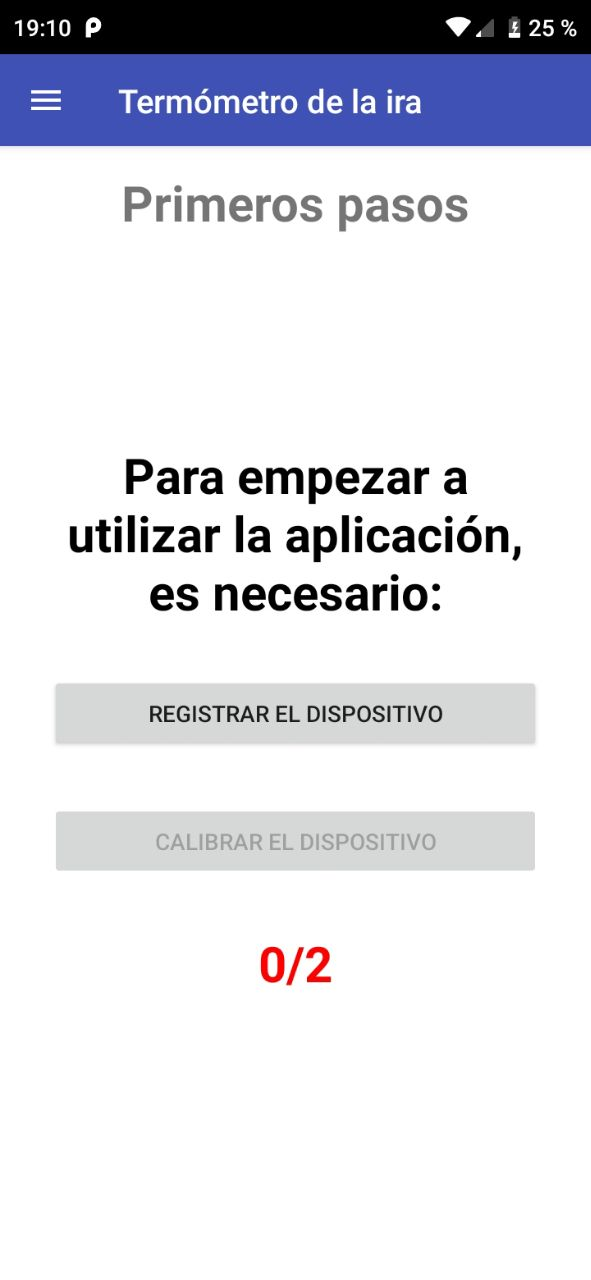
\includegraphics[scale=0.2]{Imagenes/04DescProblema/mockups/v3/android/01IndexNotCalibrated.jpg}}
        \caption[Mockup de la 3ª iteración de la pantalla de inicio cuando el dispositivo no está calibrado]{Mockup de la 3ª iteración de la pantalla de inicio cuando el dispositivo no está calibrado}
        \label{c4:fig:v3:android:01IndexNotCalibrated}
    \end{minipage}
\end{figure}

 \item Para calibrar el dispositivo, es necesario obtener los valores mínimos y máximos de las constantes fisiológicas con las que se determinarán el nivel de ira que está atravesando el paciente. Los valores mínimos se obtienen durante el sueño, tal y como se puede ver en las figuras~\ref{c4:fig:v3:android:07CalibrateSleep} y~\ref{c4:fig:v3:android:08CalibrateSleep2}. Los valores máximos se obtendrán durante una sesión de ejercicio físico que se registrará en la pantalla de la figura~\ref{c4:fig:v3:android:09CalibrateExercise}. El orden de la calibración de los valores mínimos y máximos es indiferente.
   \item Una vez se haya finalizado la calibración durante el ejercicio físico y el sueño, se cargará la que será la pantalla de la figura~\ref{c4:fig:v3:android:10IndexCalibrated}, que a partir de ahora será la nueva pantalla principal, sustituyendo a la pantalla de la figura~\ref{c4:fig:v3:android:01IndexNotCalibrated}, que al dejar de tener razón de ser pasará a dejar de ser accesible. En esta nueva pantalla principal se puede ver un icono que representa el termómetro de la ira con cinco estados correspondientes a los valores enteros entre cero y cuatro. Este icono viene acompañado de un literal con la denominación del nivel de ira siguiendo un patrón de colores similar al de un semáforo y un literal con el nivel de ira actual del paciente entre cero y cuatro. Estos elementos son comunes a las pantallas de las figuras~\ref{c4:fig:v3:android:10IndexCalibrated},~\ref{c4:fig:v3:android:11Episode1} y~\ref{c4:fig:v3:android:12Episode2}. Tras esto, en la pantalla de la figura~\ref{c4:fig:v3:android:10IndexCalibrated} se puede ver un literal en el que aparecerán el número de episodios en las últimas 24 horas y si este número de episodios es igual al día anterior o el número de episodios mayor o menor respecto al día anterior.    

\begin{figure}[H]
    \centering
    \begin{minipage}{.6\textwidth}
        \centering
        \frame{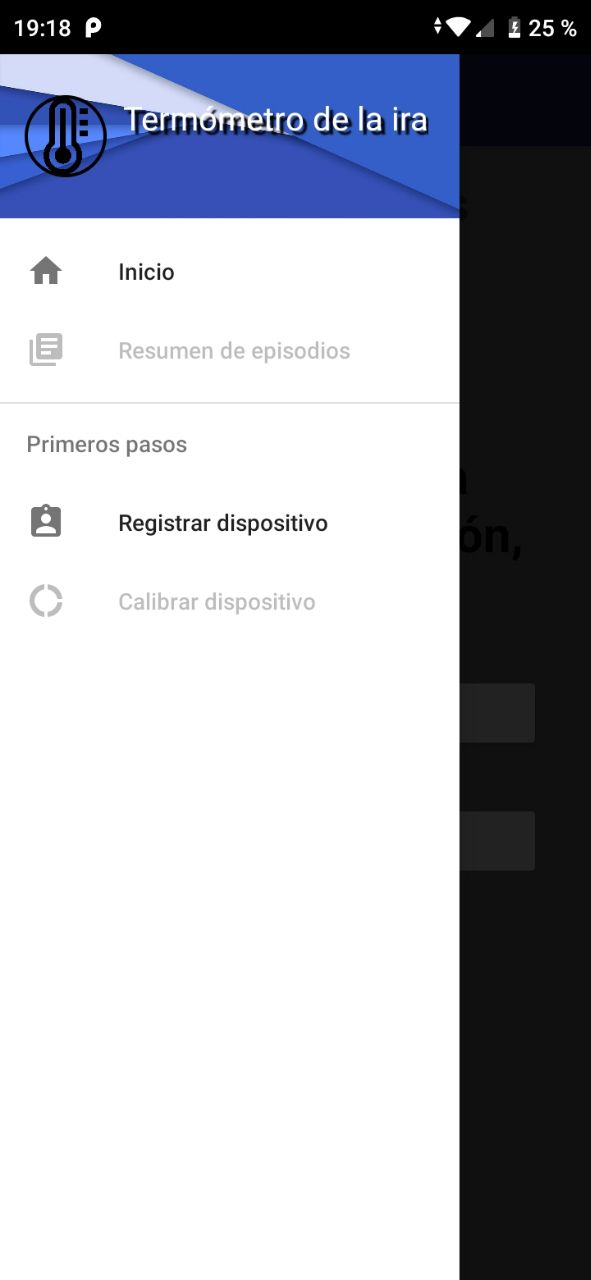
\includegraphics[scale=0.2]{Imagenes/04DescProblema/mockups/v3/android/02MenuNotCalibrated.jpg}}
        \caption[Mockup de la 3ª iteración del menú cuando el dispositivo no está calibrado]{Mockup de la 3ª iteración del menú cuando el dispositivo no está calibrado}
        \label{c4:fig:v3:android:02MenuNotCalibrated}
    \end{minipage}
\end{figure}
   

\begin{figure}[H]
    \centering
    \begin{minipage}{.6\textwidth}
        \centering
        \frame{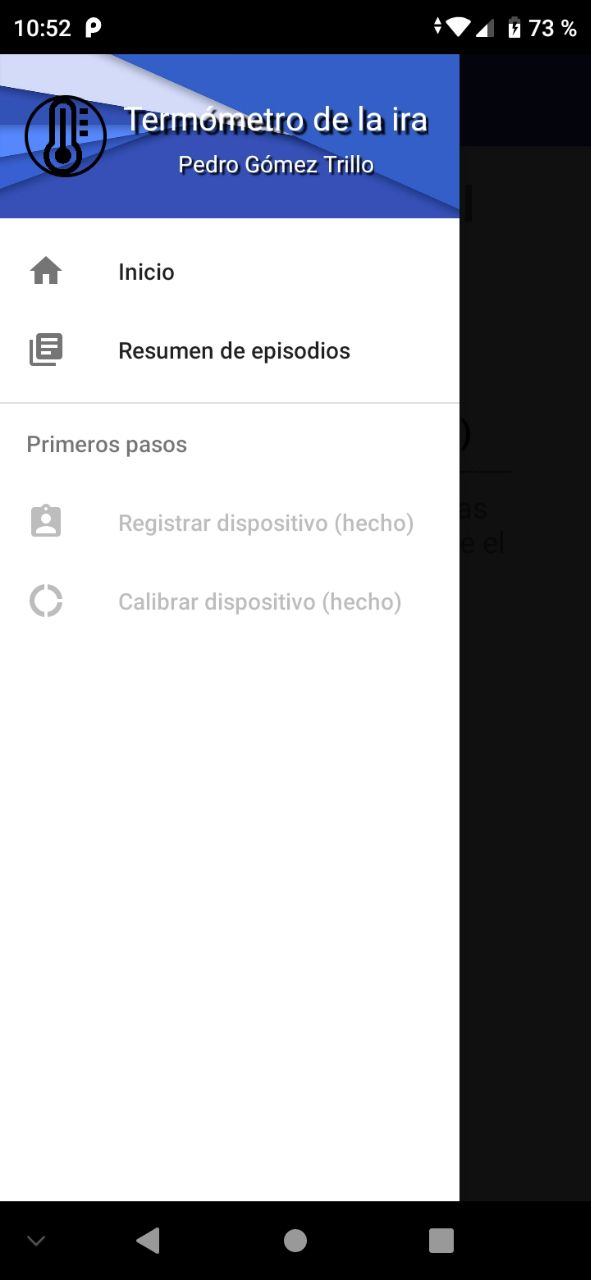
\includegraphics[scale=0.2]{Imagenes/04DescProblema/mockups/v3/android/03MenuCalibrated.jpg}}
        \caption[Mockup de la 3ª iteración del menú cuando el dispositivo está calibrado]{Mockup de la 3ª iteración del menú cuando el dispositivo está calibrado}
        \label{c4:fig:v3:android:03MenuCalibrated}
    \end{minipage}
\end{figure}

\begin{figure}[H]
    \centering
    \begin{minipage}{.6\textwidth}
        \centering
        \frame{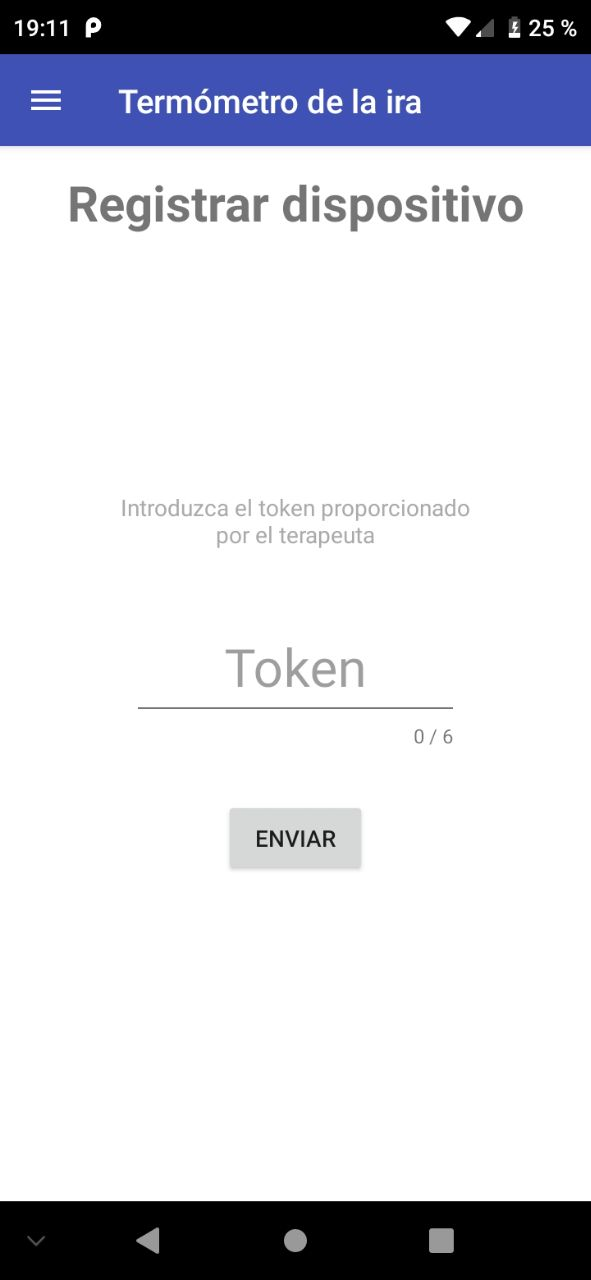
\includegraphics[scale=0.2]{Imagenes/04DescProblema/mockups/v3/android/04RegisterDevice.jpg}}
        \caption[Mockup de la 3ª iteración de la pantalla de registro del dispositivo]{Mockup de la 3ª iteración de la pantalla de registro del dispositivo}
        \label{c4:fig:v3:android:04RegisterDevice}
    \end{minipage}
\end{figure}   
    

   
\begin{figure}[H]
    \centering
    \begin{minipage}{.6\textwidth}
        \centering
        \frame{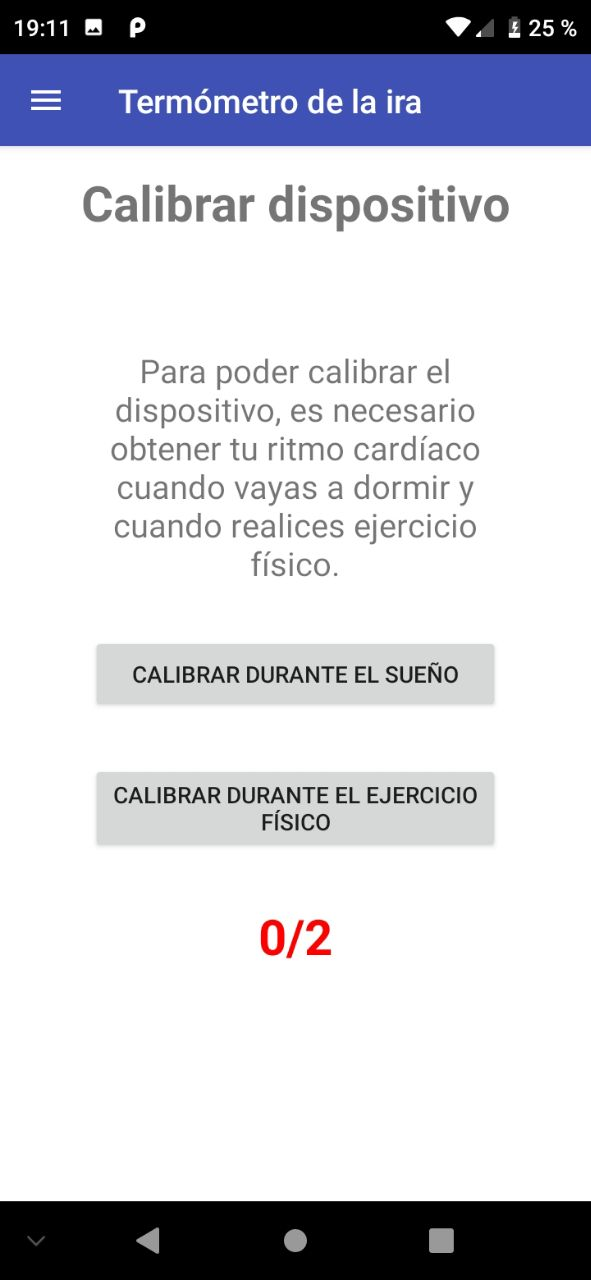
\includegraphics[scale=0.2]{Imagenes/04DescProblema/mockups/v3/android/05CalibrateDevice.jpg}}
        \caption[Mockup de la 3ª iteración de la pantalla para calibrar el dispositivo (I/II)]{Mockup de la 3ª iteración de la pantalla para calibrar el dispositivo (I/II)}
        \label{c4:fig:v3:android:05CalibrateDevice}
    \end{minipage}
\end{figure}   

\begin{figure}[H]
    \centering
    \begin{minipage}{.6\textwidth}
        \centering
        \frame{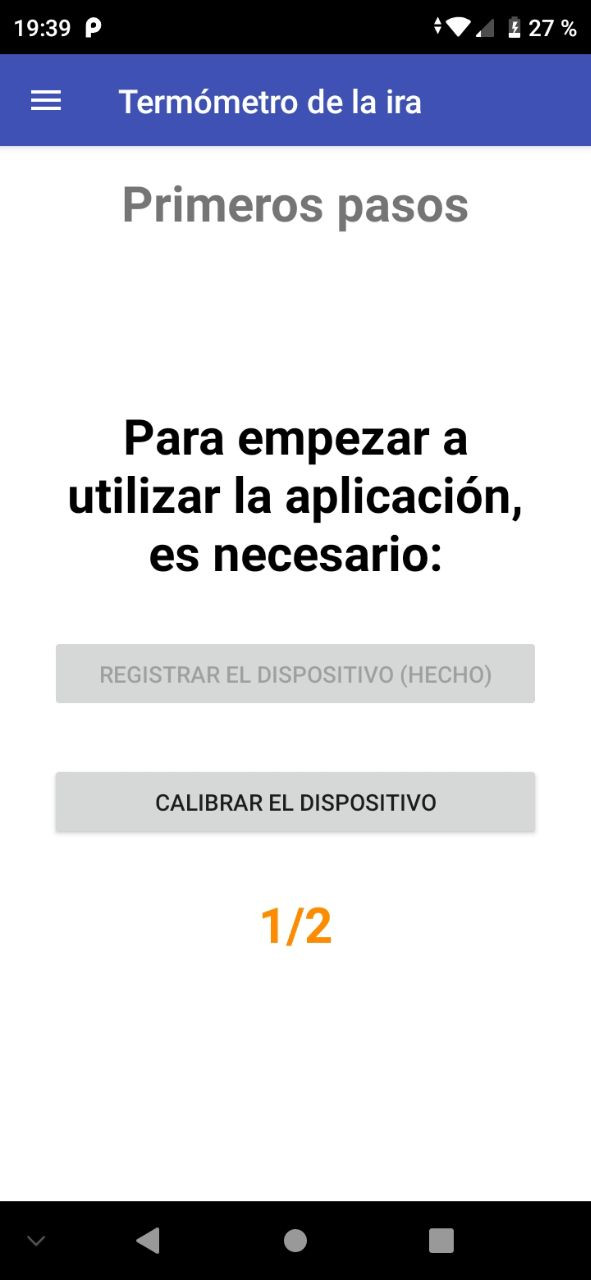
\includegraphics[scale=0.2]{Imagenes/04DescProblema/mockups/v3/android/06CalibrateDevice2.jpg}}
        \caption[Mockup de la 3ª iteración de la pantalla para calibrar el dispositivo (II/II)]{Mockup de la 3ª iteración de la pantalla para calibrar el dispositivo (II/II)}
        \label{c4:fig:v3:android:06CalibrateDevice2}
    \end{minipage}
\end{figure}

\begin{figure}[H]
    \centering
    \begin{minipage}{.6\textwidth}
        \centering
        \frame{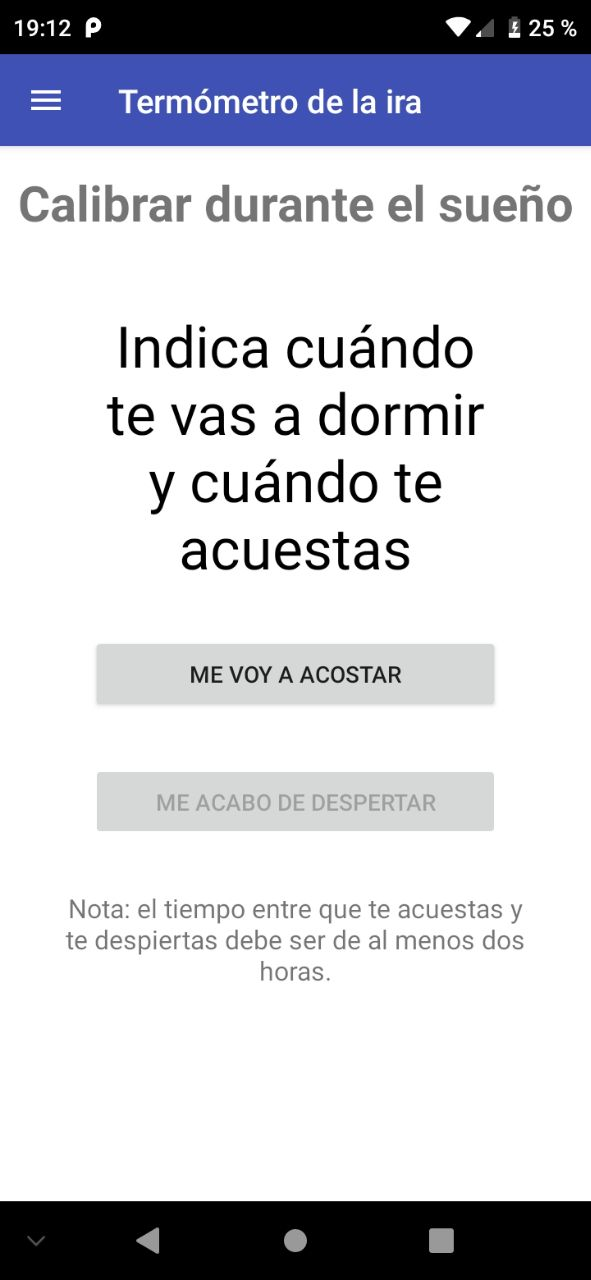
\includegraphics[scale=0.2]{Imagenes/04DescProblema/mockups/v3/android/07CalibrateSleep.jpg}}
        \caption[Mockup de la 3ª iteración de la pantalla para calibrar durante el sueño (I/II)]{Mockup de la 3ª iteración de la pantalla para calibrar durante el sueño (I/II)}
        \label{c4:fig:v3:android:07CalibrateSleep}
    \end{minipage}
\end{figure}

\begin{figure}[H]
    \centering
    \begin{minipage}{.6\textwidth}
        \centering
        \frame{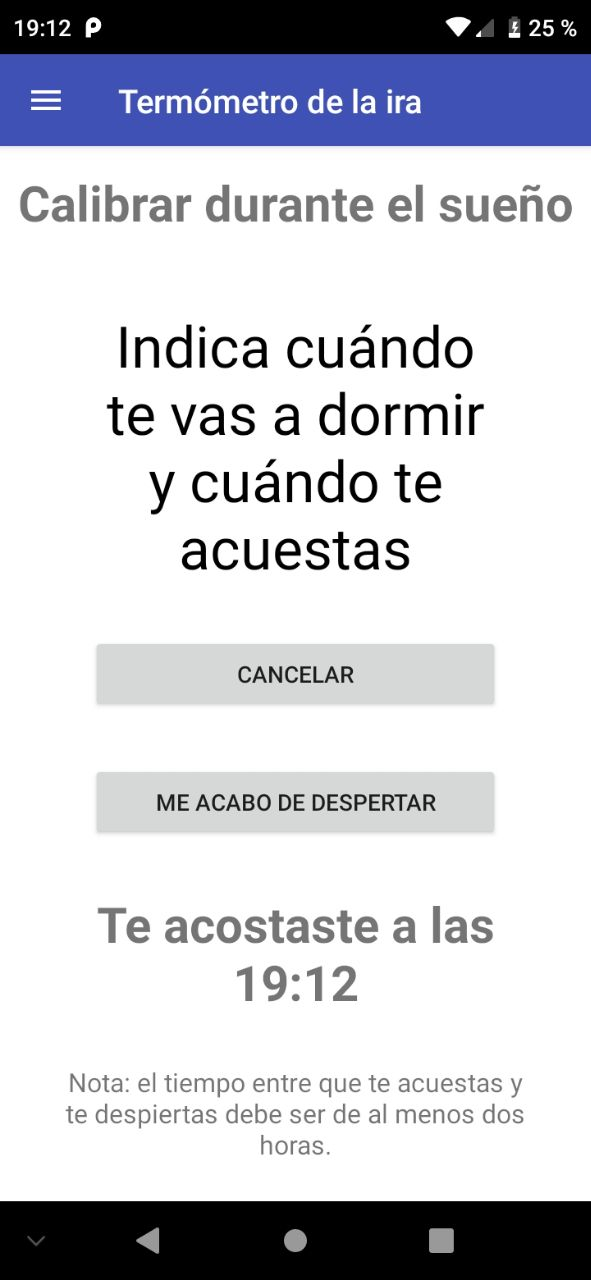
\includegraphics[scale=0.2]{Imagenes/04DescProblema/mockups/v3/android/08CalibrateSleep2.jpg}}
        \caption[Mockup de la 3ª iteración de la pantalla para calibrar durante el sueño (II/II) físico]{Mockup de la 3ª iteración de la pantalla para calibrar durante el sueño (II/II)}
        \label{c4:fig:v3:android:08CalibrateSleep2}
    \end{minipage}
\end{figure}
   
   \item La pantalla de la figura~\ref{c4:fig:v3:android:11Episode1} se cargará automáticamente cuando se inicie un episodio. En esta pantalla, el usuario deberá determinar el motivo principal de la ira entre trece opciones distintas. Una vez se haya determinado este motivo, se cargará la pantalla de la figura~\ref{c4:fig:v3:android:12Episode2}.
   \item En la pantalla de la figura~\ref{c4:fig:v3:android:12Episode2} aparecerá la pauta recomendada al paciente para reducir su nivel de ira. En caso de querer ver otra pauta, podrá descartar y cargar otra pauta pulsando sobre las fechas de la izquierda y derecha. A su vez, podrá rellenar comentarios sobre la pauta en cuestión que serán después enviados a la terapeuta para poder afinar las pautas. El botón para guardar los comentarios estará deshabilido siempre que no se detecte que el campo de texto de comentarios está relleno, acción que habilitará este botón. Una vez encontrada una pauta adecuada y esta haya sido aplicada (se presupone que el paciente siempre va a encontrar una pauta que le sea útil y que éste aplique), al pulsar sobre el botón "pauta aplicada", se cargará la pantalla de la figura~\ref{c4:fig:v3:android:13Episode3}.
   
   
\begin{figure}[H]
    \centering
    \begin{minipage}{.6\textwidth}
        \centering
        \frame{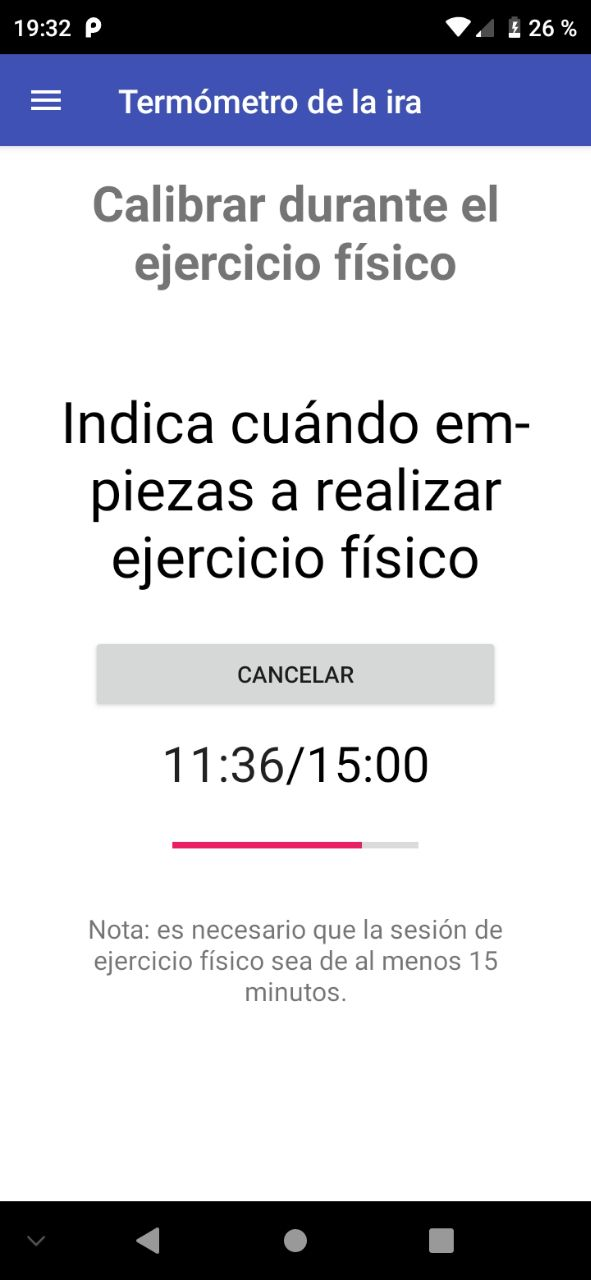
\includegraphics[scale=0.2]{Imagenes/04DescProblema/mockups/v3/android/09CalibrateExercise.jpg}}
        \caption[Mockup de la 3ª iteración de la pantalla para calibrar durante el ejercicio físico]{Mockup de la 3ª iteración de la pantalla para calibrar durante el ejercicio físico}
        \label{c4:fig:v3:android:09CalibrateExercise}
    \end{minipage}
\end{figure}   
   
   \item En la pantalla de la figura~\ref{c4:fig:v3:android:13Episode3} el usuario deberá indicar si la pauta que finalmente aplicó le resultó útil o no. Tras esto, si se detecta que el nivel de ira del paciente ha bajado a cero, se cargará la pantalla~\ref{c4:fig:v3:android:10IndexCalibrated}. En caso contrario, se cargará la pantalla~\ref{c4:fig:v3:android:12Episode2} y se seguirá este mismo ciclo hasta que se detecte que ha finalizado el episodio de ira.

   
   \item En la pantalla de las figuras~\ref{c4:fig:v3:android:14EpisodesHistory} y~\ref{c4:fig:v3:android:15EpisodesHistory2} se puede ver la búsqueda que puede hacer el usuario para ver la evolución de los episodios del paciente agrupados en intervalos de un día. Se muestran tres gráficas, con la que se puede determinar el número de episodios por día y la duración media y total de estos episodios, para que así el paciente pueda ver su evolución a lo largo del tiempo.
\end{itemize}

\paragraph{}
En este caso, a diferencia de lo que ocurre con la tercera versión de la aplicación web, debido a que se terminó esta última versión en una fecha próxima a la entrega de este trabajo combinado con el hecho de que fuese en periodo vacacional, las modificaciones que pudieran surgir fruto de la evaluación de esta versión por parte de la experta quedan relegadas al trabajo futuro.











\begin{figure}[H]
    \centering
    \begin{minipage}{.6\textwidth}
        \centering
        \frame{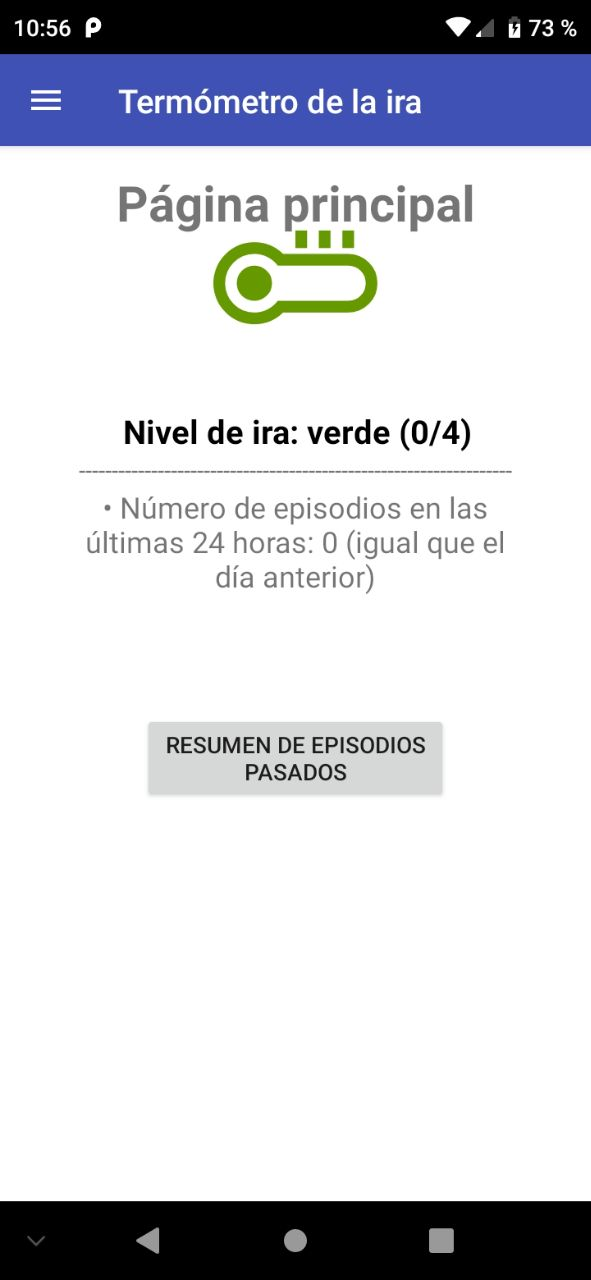
\includegraphics[scale=0.2]{Imagenes/04DescProblema/mockups/v3/android/10IndexCalibrated.jpg}}
        \caption[Mockup de la 3ª iteración de la pantalla de inicio cuando el dispositivo está calibrado]{Mockup de la 3ª iteración de la pantalla de inicio cuando el dispositivo está calibrado}
        \label{c4:fig:v3:android:10IndexCalibrated}
    \end{minipage}
\end{figure}

\begin{figure}[H]
    \centering
    \begin{minipage}{.6\textwidth}
        \centering
        \frame{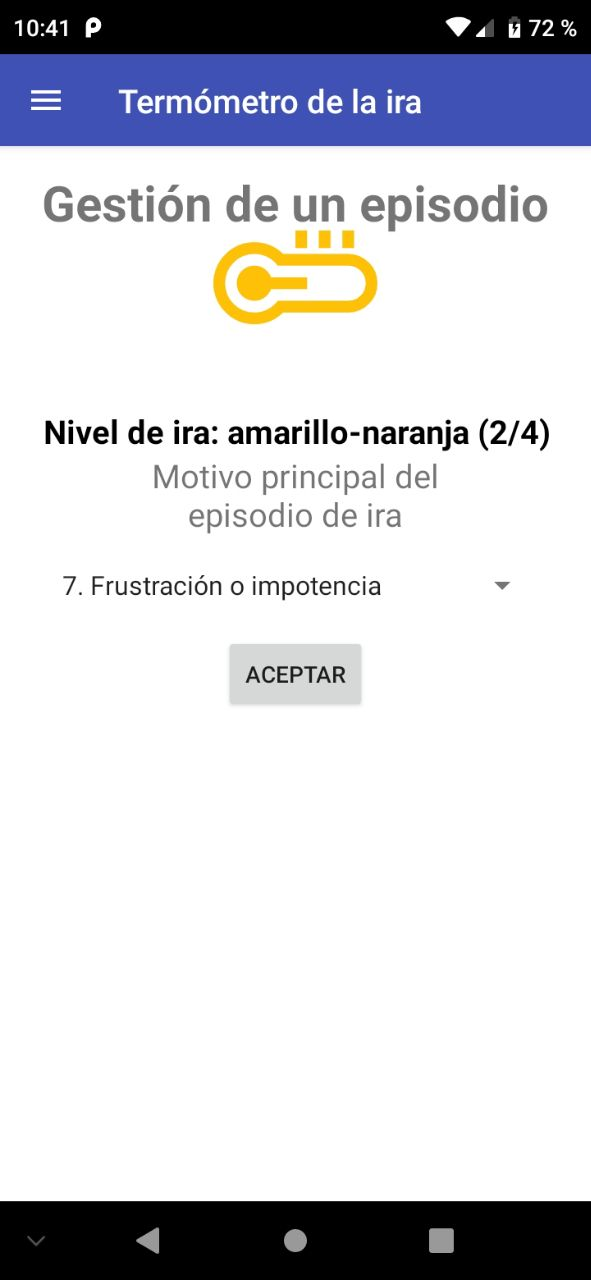
\includegraphics[scale=0.2]{Imagenes/04DescProblema/mockups/v3/android/11Episode1.jpg}}
        \caption[Mockup de la 3ª iteración de la pantalla de selección del motivo del episodio de ira]{Mockup de la 3ª iteración de la pantalla de selección del motivo del episodio de ira}
        \label{c4:fig:v3:android:11Episode1}
    \end{minipage}
\end{figure}

\begin{figure}[H]
    \centering
    \begin{minipage}{.6\textwidth}
        \centering
        \frame{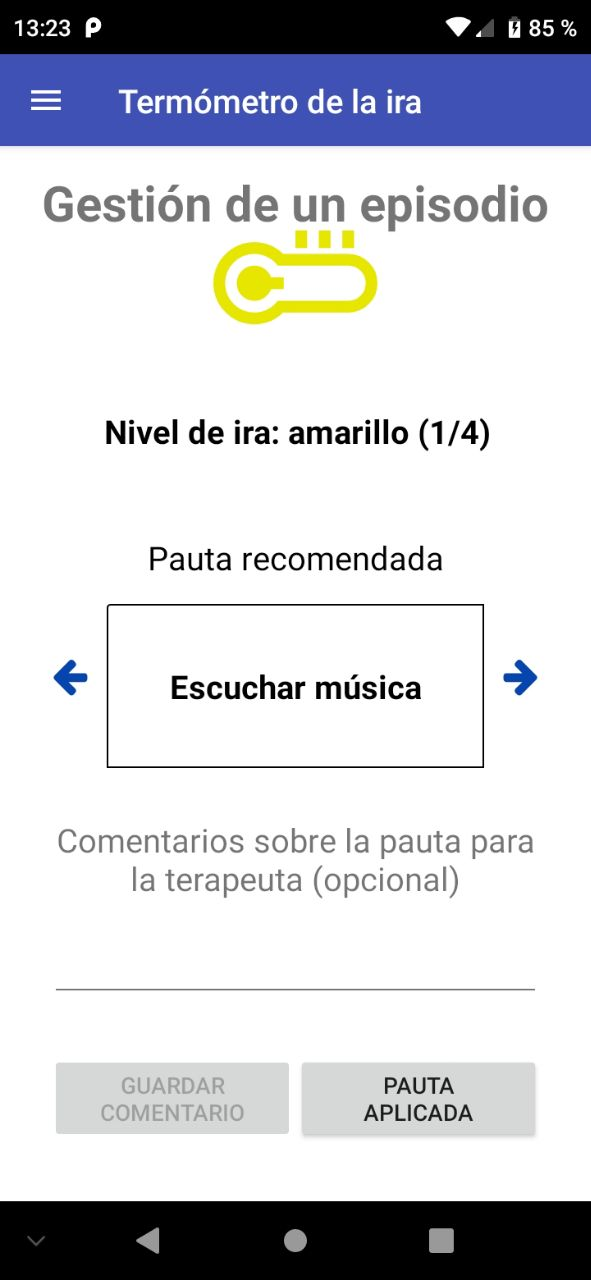
\includegraphics[scale=0.2]{Imagenes/04DescProblema/mockups/v3/android/12Episode2.jpg}}
        \caption[Mockup de la 3ª iteración de la pantalla de la pauta recomendada]{Mockup de la 3ª iteración de la pantalla de la pauta recomendada}
        \label{c4:fig:v3:android:12Episode2}
    \end{minipage}
\end{figure}

\begin{figure}[H]
    \centering
    \begin{minipage}{.6\textwidth}
        \centering
        \frame{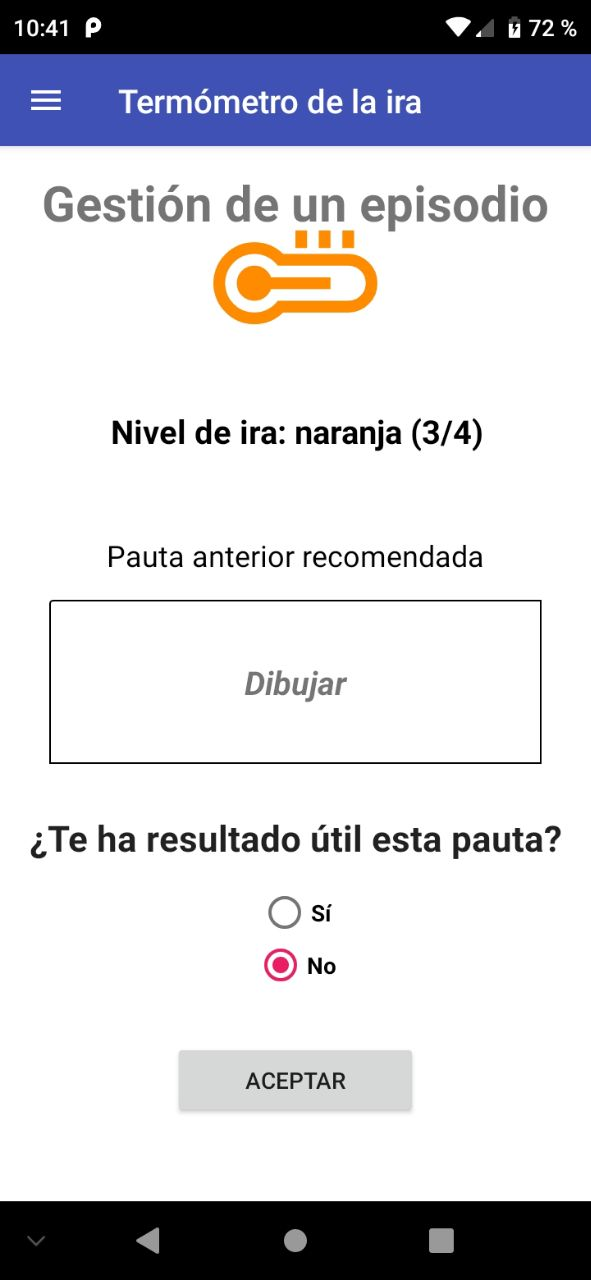
\includegraphics[scale=0.2]{Imagenes/04DescProblema/mockups/v3/android/13Episode3.jpg}}
        \caption[Mockup de la 3ª iteración de la pantalla de valoración de la pauta]{Mockup de la 3ª iteración de la pantalla de valoración de la pauta}
        \label{c4:fig:v3:android:13Episode3}
    \end{minipage}
\end{figure}

\begin{figure}[H]
    \centering
    \begin{minipage}{.6\textwidth}
        \centering
        \frame{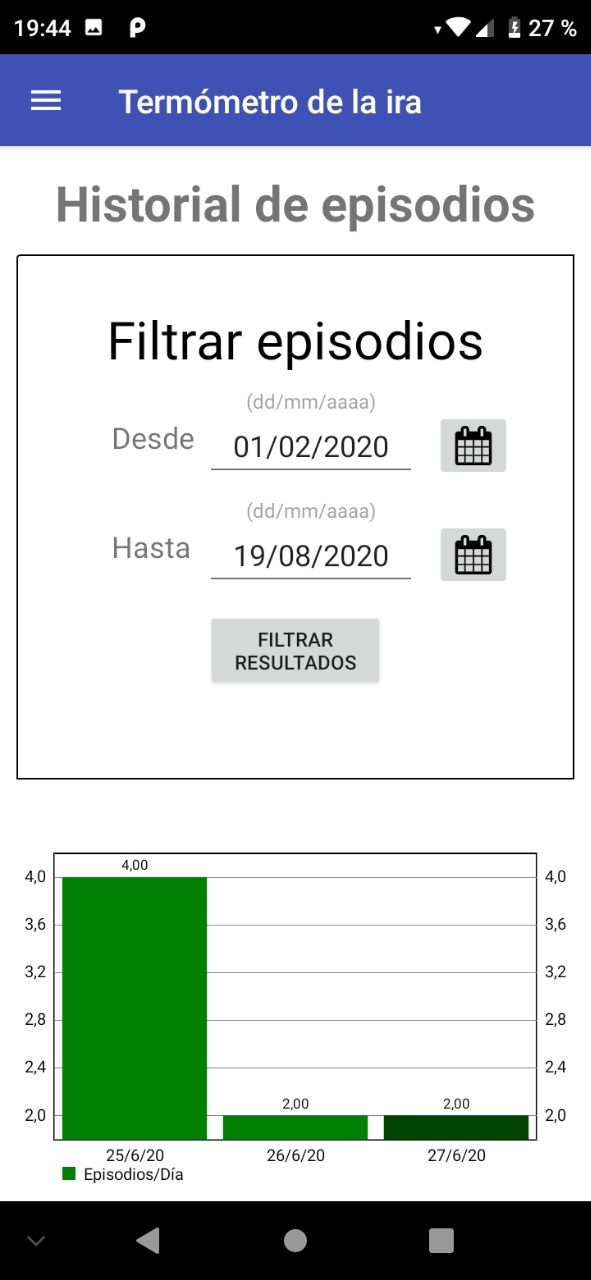
\includegraphics[scale=0.2]{Imagenes/04DescProblema/mockups/v3/android/14EpisodesHistory.jpg}}
        \caption[Mockup de la 3ª iteración de la pantalla de historial de episodios (I/II)]{Mockup de la 3ª iteración de la pantalla de historial de episodios (I/II)}
        \label{c4:fig:v3:android:14EpisodesHistory}
    \end{minipage}
\end{figure}

\begin{figure}[H]
    \centering
    \begin{minipage}{.6\textwidth}
        \centering
        \frame{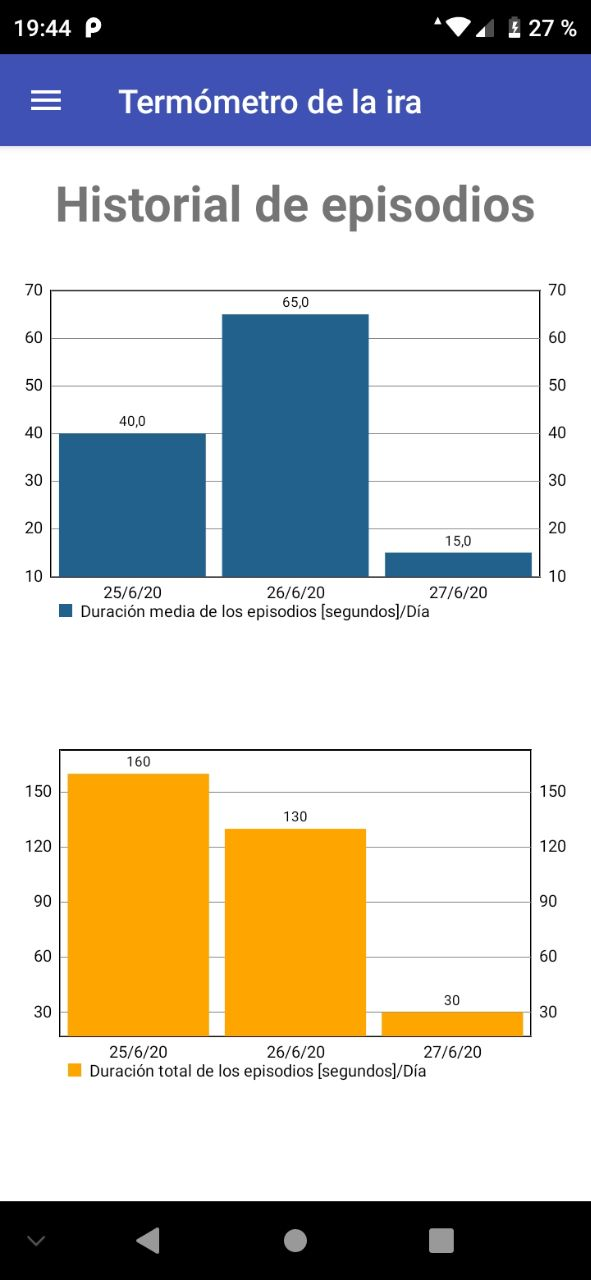
\includegraphics[scale=0.2]{Imagenes/04DescProblema/mockups/v3/android/15EpisodesHistory2.jpg}}
        \caption[Mockup de la 3ª iteración de la pantalla de historial de episodios (II/II)]{Mockup de la 3ª iteración de la pantalla de historial de episodios (II/II)}
        \label{c4:fig:v3:android:15EpisodesHistory2}
    \end{minipage}
\end{figure}

\subsubsection{Diseño de la aplicación web del terapeuta}
\paragraph{}
Para el diseño de la web, ha sido vital contar con un \textit{framework} de estilo CSS que ahorrase tiempo y sirviese para estandarizar el \textit{frontend}. Para la interfaz, se ha utilizado extensivamente las cajas. Las cajas, son una división de html con bordes grises que ha servido para agrupar elementos similares, como pueden ser los elementos secundarios de una tabla (número de registros totales, nombre de la tabla y paginadores) y la tabla en sí. Las operaciones que se realizan en la interfaz están conectadas con la base de datos de \textit{Mongo}, por lo que las operaciones \textit{CRUD} que se realizan en la interfaz, se persisten en Mongo. Las única limitación del diseño respecto a la implementación es que la web no está conectada por RabbitMQ a la aplicación Android, por lo que todos los datos son inventados y no hay un flujo de datos en tiempo real, ya que para evaluar el diseño es innecesario.

\paragraph{}
En la figura~\ref{c4:fig:v3:web:index} se puede ver la página principal de la web. En la parte superior, aparecen el número de pautas, pacientes y grupos registrados por el usuario. Cada uno de ellos redireccionaría a la página correspondiente de búsqueda de pautas, pacientes o grupos. En la parte inferior, hay un seleccionable con todos los pacientes y una serie de filtros para ver todos los episodios del paciente que se ha seleccionado en la franja temporal indicada. Tras realizar la búsqueda, se rellenaría una tabla con una fila por cada episodio. Esta lista de episodios podrán ser luego vistos uno a uno en detalle al clicar sobre los enlaces de cada fila con la palabra "ver".

\begin{figure}[H]
    \centering
    \frame{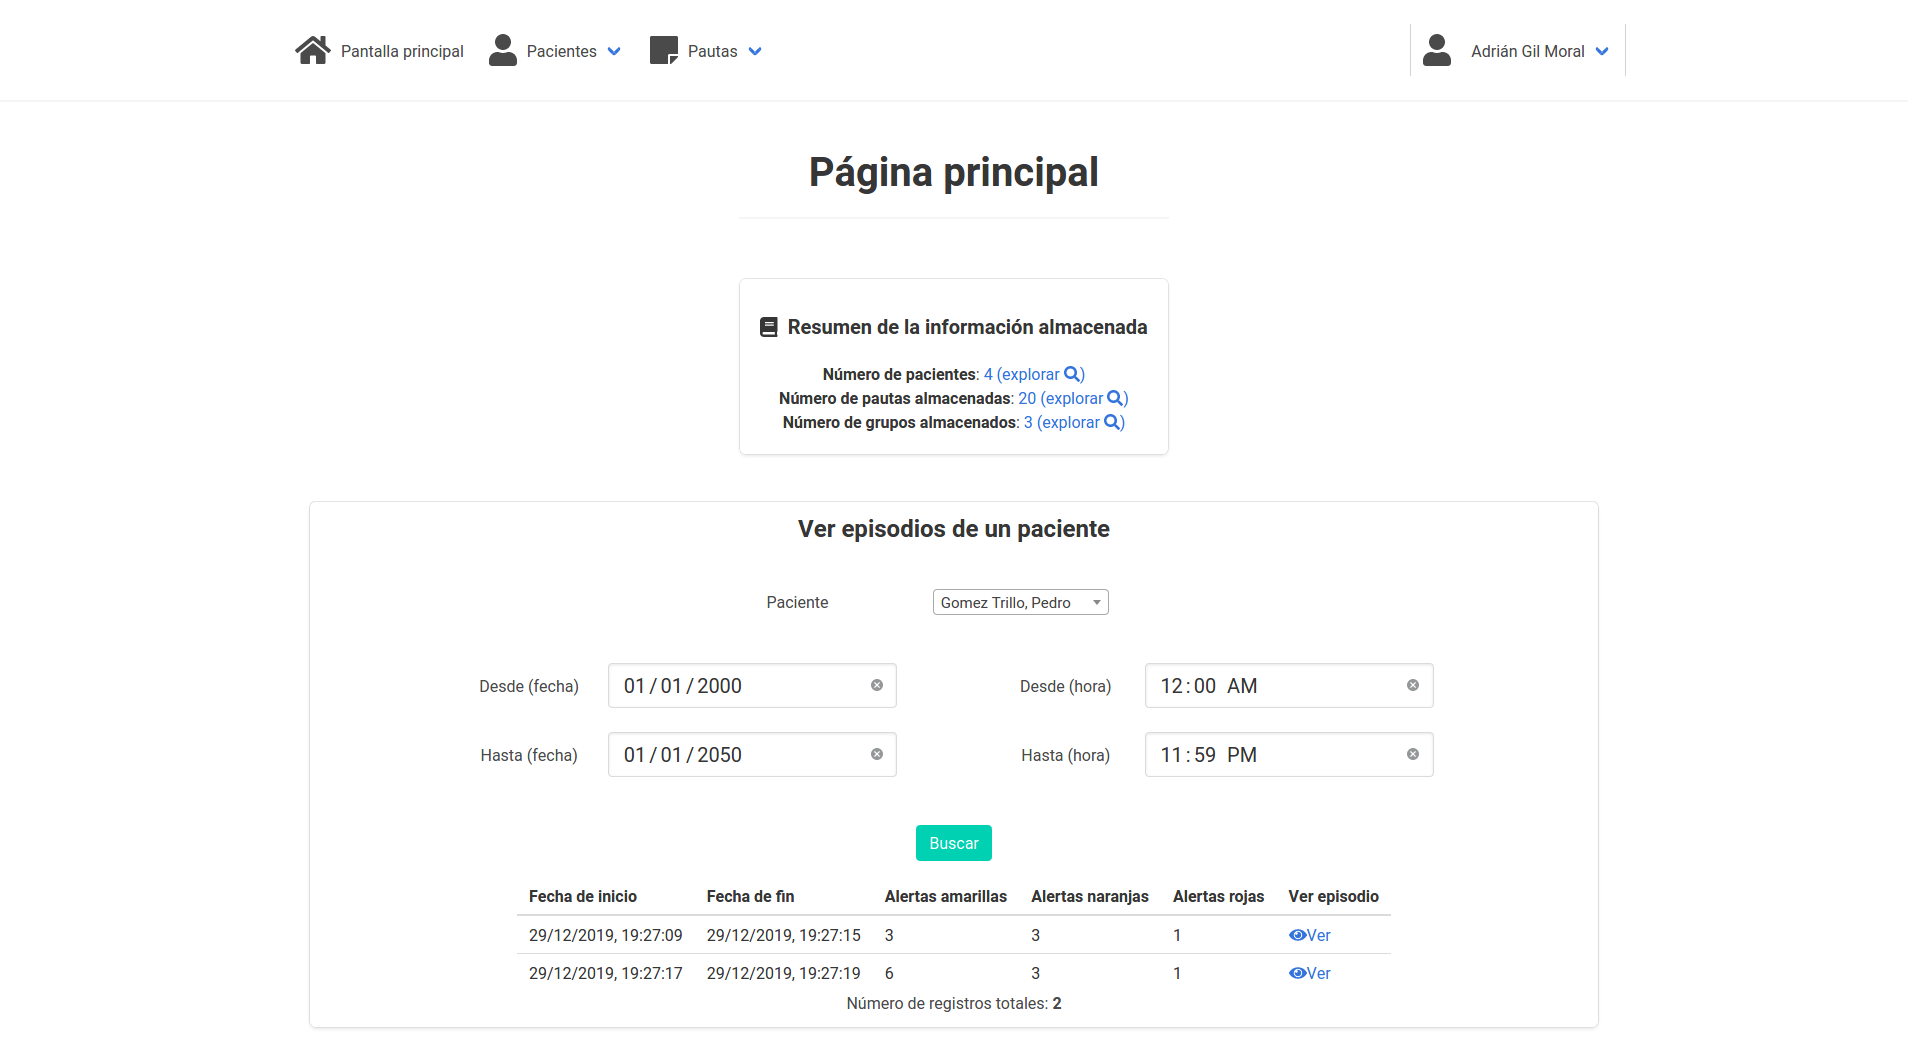
\includegraphics[scale=0.2]{Imagenes/04DescProblema/mockups/v3/web/01-index.png}}
    \caption[Mockup de la 3ª iteración de la pantalla principal de la web]{Mockup de la 3ª iteración de la pantalla principal de la web}
    \label{c4:fig:v3:web:index}
\end{figure}

\begin{figure}[H]
    \centering
    \frame{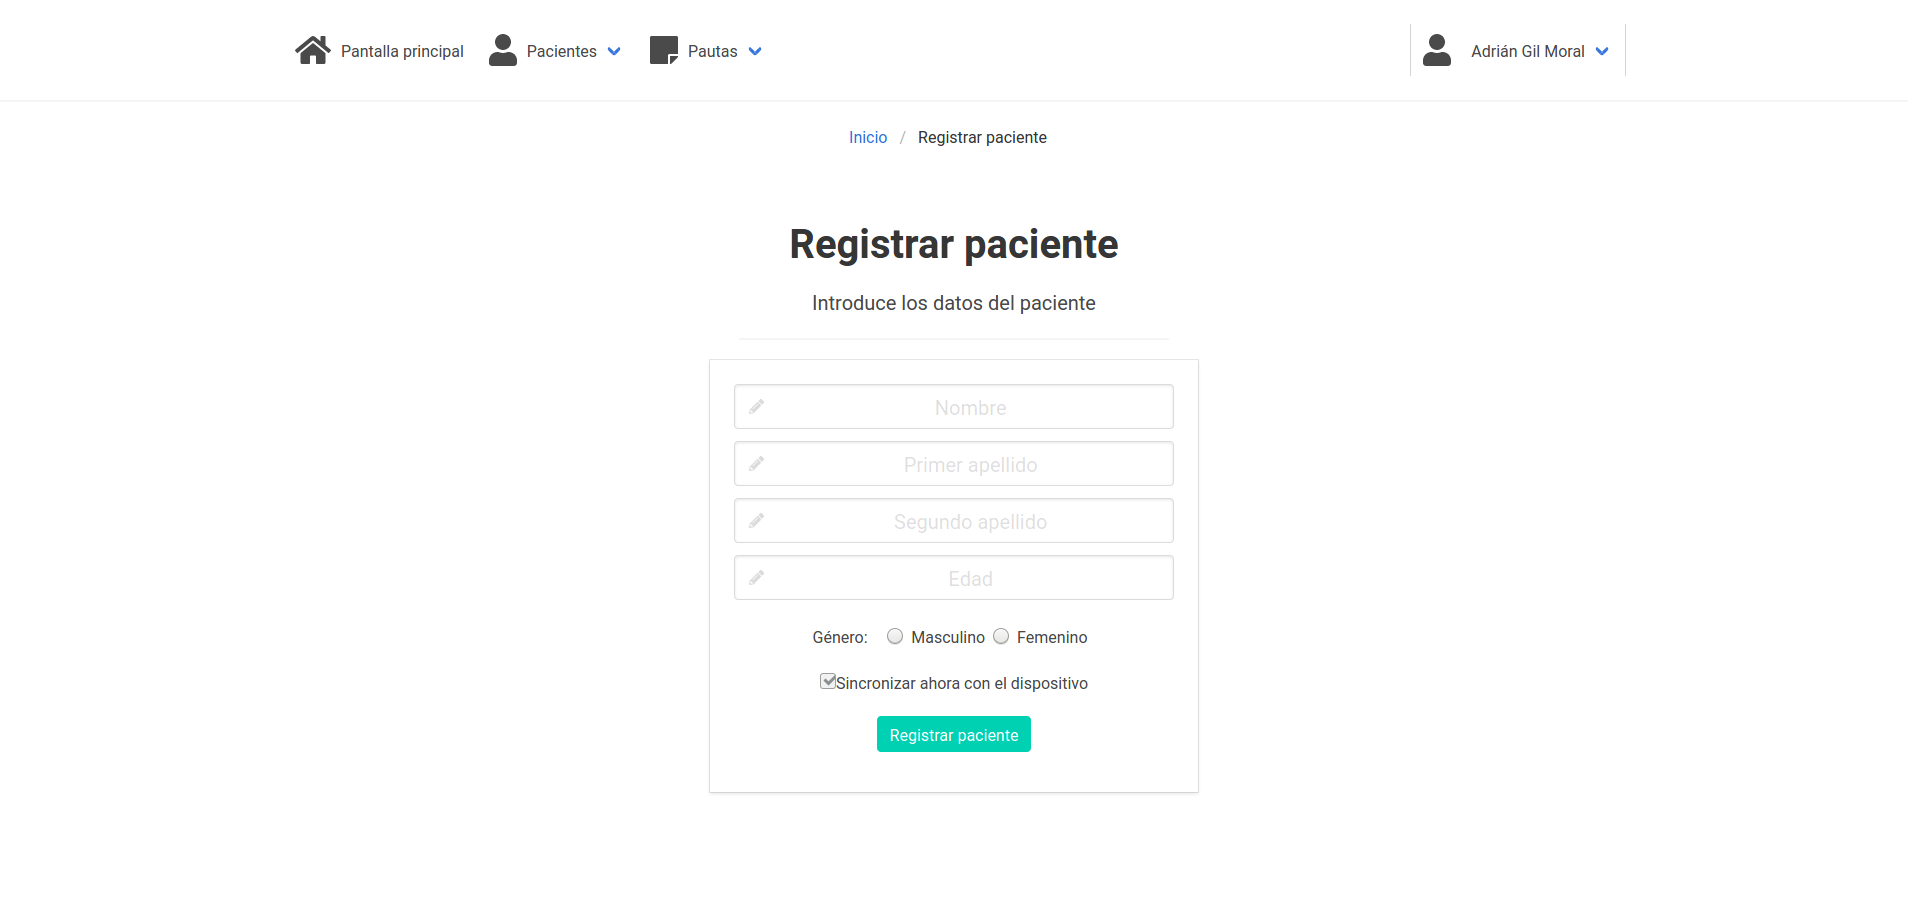
\includegraphics[scale=0.2]{Imagenes/04DescProblema/mockups/v3/web/02-registrarPaciente.png}}
    \caption[Mockup de la 3ª iteración de la pantalla de registro del paciente en la web (1/2)]{Mockup de la 3ª iteración de la pantalla de registro del paciente en la web (1/2)}
    \label{c4:fig:v3:web:registroPaciente}
\end{figure}

\paragraph{}
En la figura~\ref{c4:fig:v3:web:registroPaciente} aparece el formulario para registrar el paciente. La información obligatoria que hay que introducir es el nombre, primer apellido, edad y género del paciente. El único campo opcional es el del segundo apellido, ya que en algunos países como Inglaterra solo usan un apellido. Al pulsar sobre el botón para registrar paciente, este primer formulario se desplazará a la izquierda y todos los campos se volverán no editables, tal y como se ve en la figura~\ref{c4:fig:v3:web:registroPaciente2}. En paralelo, se mostrará un mensaje indicando a la terapeuta el \textit{token} que el paciente que se está registrando debe introducir en la aplicación móvil. Por motivos de seguridad, se da un plazo de cinco minutos, por lo que se espera que el paciente acuda a la consulta con su dispositivo móvil y se descargue la aplicación en la consulta. En caso de haber introducido algún dato erróneo, se cancelaría el proceso de sincronización y los campos del formulario se volverían editables. En el caso de que sí se produzca la sincronización con el dispositivo móvil, se redireccionaría a la página principal y se indicaría mediante un mensaje que se ha completado correctamente el registro del usuario.

\begin{figure}[H]
    \centering
    \frame{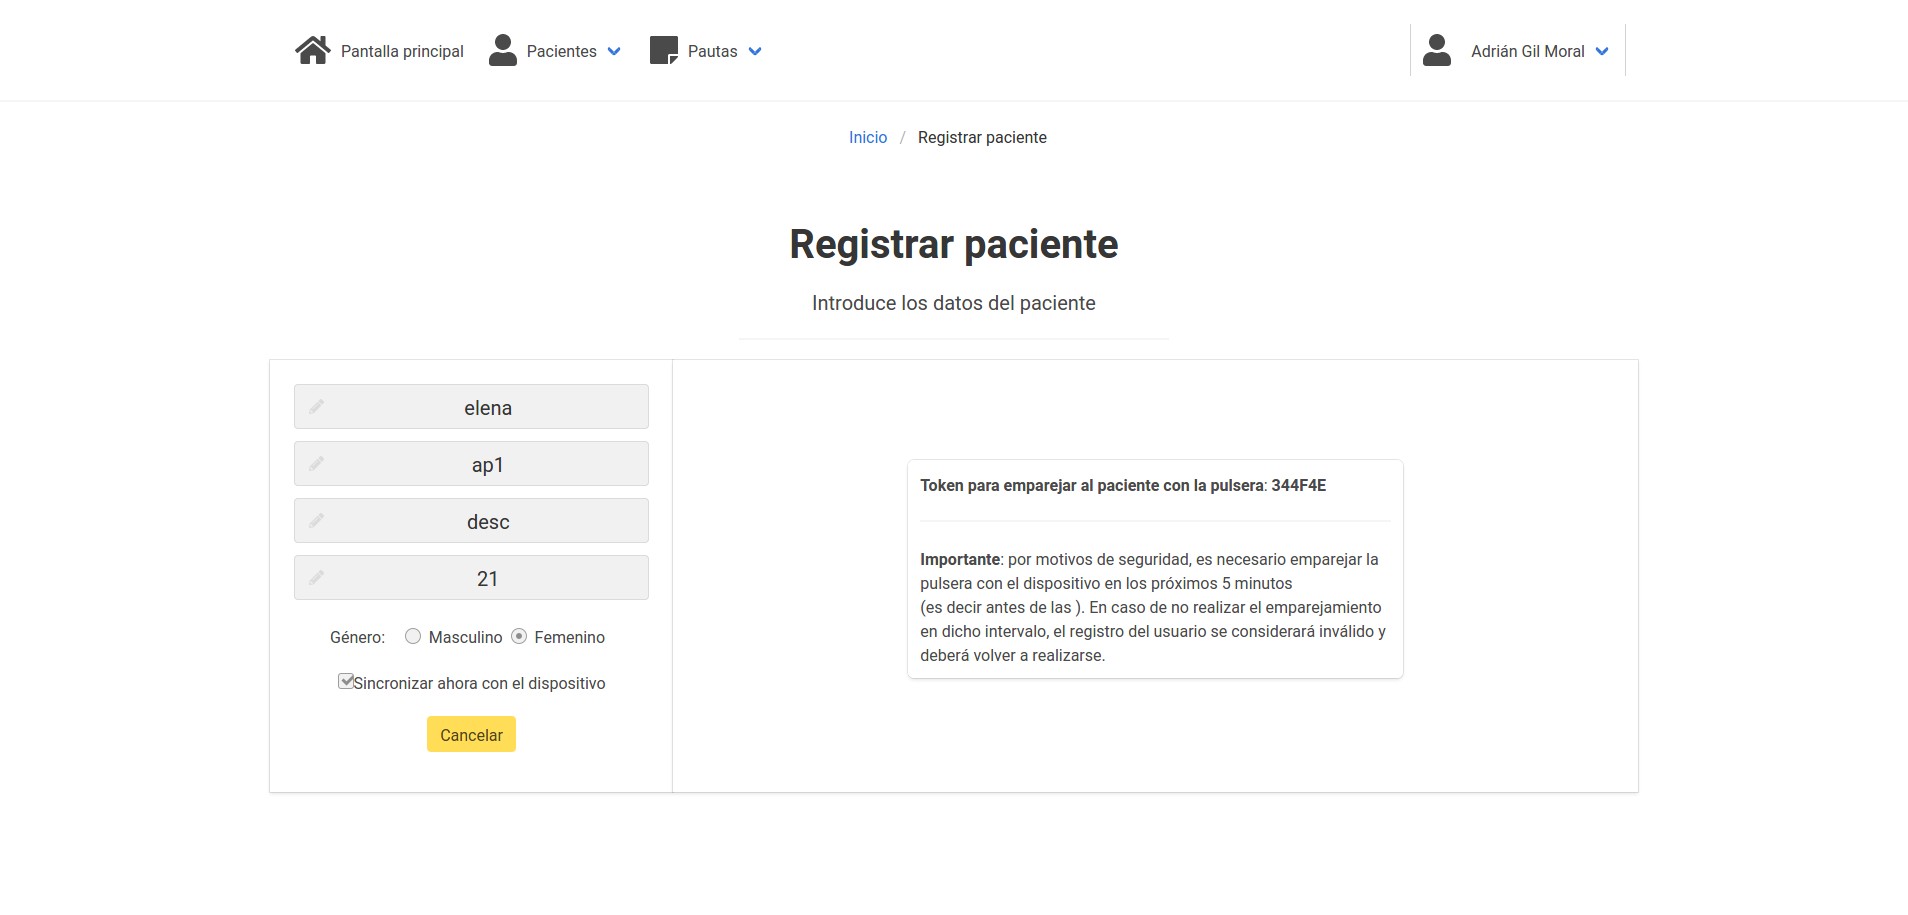
\includegraphics[scale=0.2]{Imagenes/04DescProblema/mockups/v3/web/03-registrarPaciente-2.png}}
    \caption[Mockup de la 3ª iteración de la pantalla de registro del paciente en la web (2/2)]{Mockup de la 3ª iteración de la pantalla de registro del paciente en la web (2/2)}
    \label{c4:fig:v3:web:registroPaciente2}
\end{figure}

\begin{figure}[H]
    \centering
    \frame{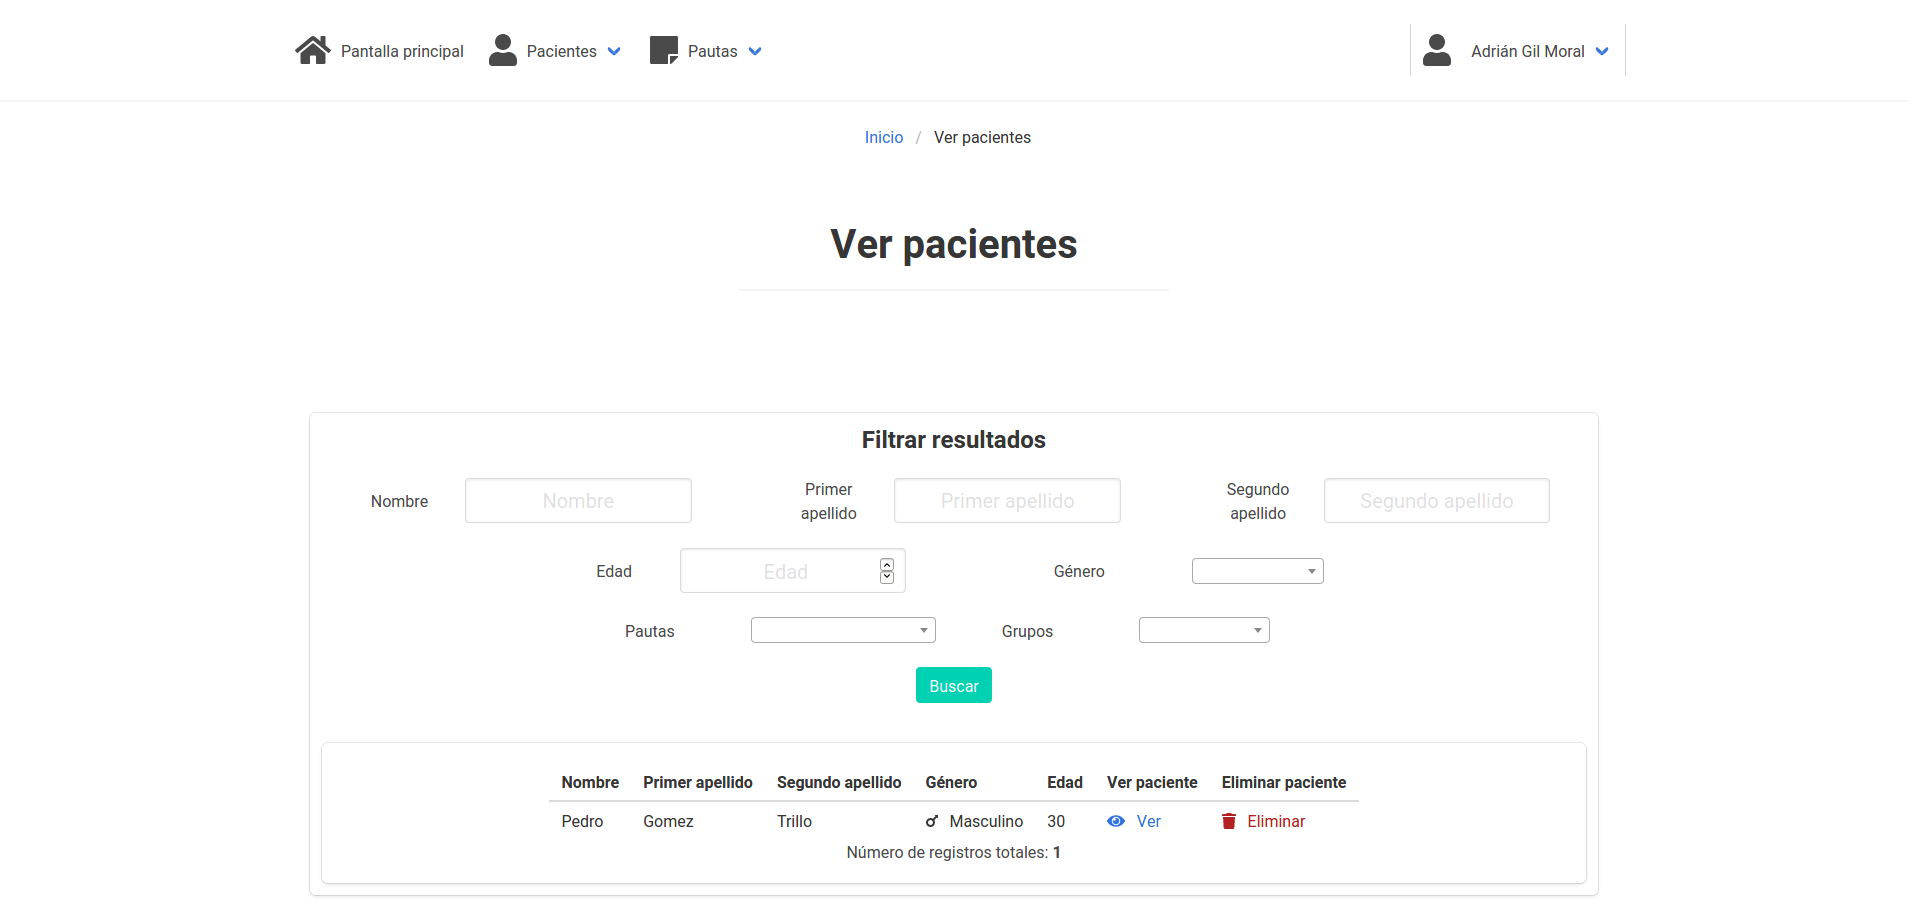
\includegraphics[scale=0.2]{Imagenes/04DescProblema/mockups/v3/web/04-verPacientes.png}}
    \caption[Mockup de la 3ª iteración de la pantalla para ver pacientes en la web]{Mockup de la 3ª iteración de la pantalla para ver pacientes en la web (2/2)}
    \label{c4:fig:v3:web:verPacientes}
\end{figure}

\paragraph{}
En la figura~\ref{c4:fig:v3:web:verPacientes} se encuentra un buscador genérico de pacientes. Se puede buscar a los pacientes por nombre, primer apellido, segundo apellido, edad, género y pautas que tenga asociadas. Tras realizar la búsqueda, debajo de estos filtros se rellenaría la tabla con los registros de todos los pacientes que coincidan con dichos criterios. Si no se rellena ninguno de los campos, se mostrarían todos los pacientes almacenados. Cada fila incluye un enlace para ver la información detallada de cada paciente. A su vez, es desde esta pantalla desde la que se pueden borrar pacientes. Antes de realizarse un borrado de un paciente, aparecería una ventana emergente como la que se ve en la figura~\ref{c4:fig:v3:web:ventanaEmergente} con la información del registro que se eliminaría. Esta ventana es análoga a la que se mostraría antes del borrado de pautas o grupos. En caso de pulsar aceptar, se realizaría un borrado físico de dicho registro.

\begin{figure}[H]
    \centering
    \frame{\includegraphics[scale=0.2]{Imagenes/04DescProblema/mockups/v3/web/04-verPacientes-2.png}}
    \caption[Mockup de la 3ª iteración de una ventana emergente en la web]{Mockup de la 3ª iteración de una ventana emergente en la web}
    \label{c4:fig:v3:web:ventanaEmergente}
\end{figure}

\paragraph{}
En la figura~\ref{c4:fig:v3:web:verPaciente} se puede ver la información de un paciente. En esta pantalla, la información es no editable, pero se incluyen enlaces para editar la información personal del paciente, enlazar pautas al paciente o registrar una nueva pauta para el paciente dado. La única excepción a esta regla es que se pueden desvincular pautas sin salir de esta pantalla. El motivo por el que se tomó esta decisión es porque si no, se necesitaría incluir una pantalla extra de profundidad para editar las pautas, lo que se consideraba que podría ser capcioso para el usuario.

\begin{figure}[H]
    \centering
    \frame{\includegraphics[scale=0.2]{Imagenes/04DescProblema/mockups/v3/web/05-verPaciente.png}}
    \caption[Mockup de la 3ª iteración de la pantalla para ver un paciente en la web]{Mockup de la 3ª iteración de la pantalla para ver un paciente en la web}
    \label{c4:fig:v3:web:verPaciente}
\end{figure}

\paragraph{}
En la figura~\ref{c4:fig:v3:web:modificarPaciente} se puede ver cómo se podría modificar la información personal del paciente. La información que se muestra es el formulario de registro de paciente pero estableciendo como valores por defecto de los campos (todos ellos editables) los valores del paciente. En caso de pulsar sobre el botón volver, se cargará la página que se encuentre por encima en la jerarquía, que en este caso es la página para ver la información del paciente. Al pulsarlo, no se guardarán las modificaciones que se hayan hecho en esta pantalla. En caso de modificar dicho registro y de pulsar sobre guardar, se volvería a la pantalla para ver el paciente en cuestión incluyendo un mensaje flotante para indicar que el paciente se ha modificado correctamente.

\paragraph{}
En la figura~\ref{c4:fig:v3:web:nuevaPautaPaciente} aparece la pantalla que se mostraría al clicar sobre el botón "registrar una nueva pauta" en la pantalla para ver el paciente. El formulario que aparece es el mismo que para registrar una nueva pauta, solo que en este caso la pauta al registrarse se vincularía directamente al paciente en cuestión.

\paragraph{}
En la figura~\ref{c4:fig:v3:web:enlazarPautaPaciente} se puede ver la pantalla que se carga al clicar sobre el botón "enlazar pautas" en la pantalla para ver el paciente. Es un formulario de búsqueda de todas las pautas en la que debajo aparece la lista de pautas que coinciden con los parámetros de búsqueda. Esta tabla incluye una columna con una caja seleccionable por cada fila (siendo, a su vez, una pauta por fila). Al pulsar sobre el botón "enlazar pautas", se vincularían las pautas seleccionadas al paciente en el que se haya hecho clic en el botón de "enlazar pautas". La información de este paciente aparece a su vez en la parte superior de la página. Por último, como en caso de que haya más registros en la tabla que el límite de filas por tabla que se haya establecido, se mostrará debajo de la tabla un seleccionable con todas las páginas de la tabla. Al cambiar el número de página de las tablas, se actualizarán los registros de la tabla. Estos marcadores se incluyen en todas las tablas de la web, pero solo se muestran al usuario si hay más de una página.

\begin{figure}[H]
    \centering
    \frame{\includegraphics[scale=0.2]{Imagenes/04DescProblema/mockups/v3/web/06-verPaciente-modificar.png}}
    \caption[Mockup de la 3ª iteración de la pantalla para modificar un paciente en la web]{Mockup de la 3ª iteración de la pantalla para modificar un paciente en la web}
    \label{c4:fig:v3:web:modificarPaciente}
\end{figure}

\paragraph{}
En la figura~\ref{c4:fig:v3:web:registrarPauta} aparece la pantalla para registrar una pauta. Los datos obligatorios son nombre de la pauta (que será el literal que le aparezca al usuario en el dispositivo móvil) e intensidades de la ira asociadas. De manera optativa, se puede incluir una descripción. Esta descripción sólo la visualizará el terapeuta.

\begin{figure}[H]
    \centering
    \frame{\includegraphics[scale=0.2]{Imagenes/04DescProblema/mockups/v3/web/06-verPaciente-nuevaPauta.png}}
    \caption[Mockup de la 3ª iteración de la pantalla para crear una nueva para pauta para un paciente en la web]{Mockup de la 3ª iteración de la pantalla para crear una nueva para pauta para un paciente en la web}
    \label{c4:fig:v3:web:nuevaPautaPaciente}
\end{figure}

\begin{figure}[H]
    \centering
    \frame{\includegraphics[scale=0.2]{Imagenes/04DescProblema/mockups/v3/web/07-verPaciente-enlazarPauta.png}}
    \caption[Mockup de la 3ª iteración de la pantalla para enlazar una para pauta para un paciente en la web]{Mockup de la 3ª iteración de la pantalla para enlazar una para pauta para un paciente en la web}
    \label{c4:fig:v3:web:enlazarPautaPaciente}
\end{figure}




\paragraph{}
En la figura~\ref{c4:fig:v3:web:episodio} se puede ver la información detallada de un episodio de un paciente. Esto incluye el histograma con el nivel de alerta y una tabla en la que aparece el nivel de alerta en cada momento, la pauta que se le recomendó al paciente, si la siguió o no y los comentarios opcionales del paciente.

\paragraph{}
En la figura~\ref{c4:fig:v3:web:verPautas} se encuentra un formulario de búsqueda de pautas por nombre, descripción, intentisidades y pacientes y grupos asociados. En la parte inferior, se encuentra una tabla con los resultados de la búsqueda de pautas. Esta es la única pantalla desde la que se pueden eliminar pautas.

\paragraph{}
En la figura~\ref{c4:fig:v3:web:verPauta} se encuentra la información de una pauta. Se incluyen los datos de la pauta, la tabla de paciente que hacen uso de la pauta y la tabla de grupos que incluyen esta pauta. Estas dos últimas pautas incluyen una columna para desvincular cualquiera de los registros de la pauta en cuestión así como enlaces para vincular la pauta a nuevos pacientes y/o grupos.

\begin{figure}[H]
    \centering
    \frame{\includegraphics[scale=0.2]{Imagenes/04DescProblema/mockups/v3/web/08-registrarPauta.png}}
    \caption[Mockup de la 3ª iteración de la pantalla para registrar una nueva pauta en la web]{Mockup de la 3ª iteración de la pantalla para registrar una nueva pauta en la web}
    \label{c4:fig:v3:web:registrarPauta}
\end{figure}

\begin{figure}[H]
    \centering
    \frame{\includegraphics[scale=0.2]{Imagenes/04DescProblema/mockups/v3/web/09-verEpisodio.png}}
    \caption[Mockup de la 3ª iteración de la pantalla para ver un episodio en la web]{Mockup de la 3ª iteración de la pantalla para ver un episodio en la web}
    \label{c4:fig:v3:web:episodio}
\end{figure}

\paragraph{}
Al pulsar sobre el botón "editar" en la pantalla~\ref{c4:fig:v3:web:verPauta}, se cargaría la pantalla de la figura~\ref{c4:fig:v3:web:editarPauta}. Esta pantalla incluye el formulario que se utilizó para registrar la pauta precargado con los datos de la pauta que se pretende modificar.

\paragraph{}
Al pulsar el botón "enlazar un nuevo paciente" se cargaría la pantalla~\ref{c4:fig:v3:web:enlazarPautaPacientes}. Esta pantalla cuenta con un formulario de búsqueda de pacientes precedido por una tabla con los pacientes que resulten de la búsqueda. La primera columna de dicha tabla con la información de los pacientes sería una caja seleccionable por fila. Al pulsar sobre el botón para enlazar pauta a pacientes, se vincularía dicha pauta a los pacientes seleccionados.

\paragraph{}
Al pulsar el botón "enlazar un nuevo grupo" se cargaría la pantalla~\ref{c4:fig:v3:web:enlazarPautaGrupos}. Esta página incluye un formulario de búsqueda de grupos y una tabla con los resultados de búsqueda. Su primera columna es una caja seleccionable por fila. Al pulsar sobre el botón para enlazar pauta a pacientes, se vincularía dicha pauta a los pacientes seleccionados.

\paragraph{}
En la pantalla~\ref{c4:fig:v3:web:editarPauta}, se puede ver el formulario de registro de la pauta con los valores que tenga la pauta. Si se clica sobre volver, se cargaría la página para ver la pauta en cuestión y se perderían los cambios. Al dar clic en modificar, se persistirían los cambios.

\begin{figure}[H]
    \centering
    \frame{\includegraphics[scale=0.2]{Imagenes/04DescProblema/mockups/v3/web/10-verPautas.png}}
    \caption[Mockup de la 3ª iteración de la pantalla para ver pautas en la web]{Mockup de la 3ª iteración de la pantalla para ver pautas en la web}
    \label{c4:fig:v3:web:verPautas}
\end{figure}

\begin{figure}[H]
    \centering
    \frame{\includegraphics[scale=0.2]{Imagenes/04DescProblema/mockups/v3/web/11-verPauta.png}}
    \caption[Mockup de la 3ª iteración de la pantalla para ver una pauta en la web]{Mockup de la 3ª iteración de la pantalla para ver una pauta en la web}
    \label{c4:fig:v3:web:verPauta}
\end{figure}

\begin{figure}[H]
    \centering
    \frame{\includegraphics[scale=0.2]{Imagenes/04DescProblema/mockups/v3/web/11-verPauta-enlazarPaciente.png}}
    \caption[Mockup de la 3ª iteración de la pantalla para enlazar una pauta a pacientes en la web]{Mockup de la 3ª iteración de la pantalla para enlazar una pauta a pacientes en la web}
    \label{c4:fig:v3:web:enlazarPautaPacientes}
\end{figure}

\paragraph{}
En la pantalla~\ref{c4:fig:v3:web:registrarGrupo}, se registraría un grupo de pautas. En este formulario se incluye directamente un seleccionable en el que se pueden marcar varias opciones con todas las pautas almacenadas que formarán parte del grupo.

%TODO: revisar con pantallazos de la versión final y con los cambios que aparecen en el correo.
\paragraph{}
Tras brindarle a la experta los credenciales necesarios para poder acceder a la web, las respuestas referentes a este diseño fueron muy positivas. Las únicas modificaciones que fue necesario realizar fue la inclusión de un cuarto nivel de posibles estados en el termómetro de la ira y agrupar las columnas de nombre y apellidos de los pacientes en una única celda.

\begin{figure}[H]
    \centering
    \frame{\includegraphics[scale=0.2]{Imagenes/04DescProblema/mockups/v3/web/11-verPauta-enlazarGrupo.png}}
    \caption[Mockup de la 3ª iteración de la pantalla para enlazar una pauta a grupos en la web]{Mockup de la 3ª iteración de la pantalla para enlazar una pauta a grupos en la web}
    \label{c4:fig:v3:web:enlazarPautaGrupos}
\end{figure}

\begin{figure}[H]
    \centering
    \frame{\includegraphics[scale=0.2]{Imagenes/04DescProblema/mockups/v3/web/11-verPauta-editar.png}}
    \caption[Mockup de la 3ª iteración de la pantalla para editar una pauta en la web]{Mockup de la 3ª iteración de la pantalla para enlazar una pauta en la web}
    \label{c4:fig:v3:web:editarPauta}
\end{figure}

\begin{figure}[H]
    \centering
    \frame{\includegraphics[scale=0.2]{Imagenes/04DescProblema/mockups/v3/web/12-registrarGrupo.png}}
    \caption[Mockup de la 3ª iteración de la pantalla para registrar un grupo en la web]{Mockup de la 3ª iteración de la pantalla para registrar un grupo en la web}
    \label{c4:fig:v3:web:registrarGrupo}
\end{figure}

\section{Implementación}
\label{c4:sec:impl}
\paragraph{}
En este trabajo, se ha diseñado por un lado una aplicación Android (cuarto elemento de la figura~\ref{c4:fig:dfd}) que utilizarán los pacientes (primer elemento de la figura~\ref{c4:fig:dfd}) y una web que utilizarán los terapeutas (sexto elemento de la figura~\ref{c4:fig:dfd}). En la aplicación Android, a partir del ritmo cardíaco, la actividad electrodérmica de la piel y la aceleración, se determinará en tiempo real el nivel de ira de un paciente en una escala de cero a cuatro. La aceleración y la actividad electrodérmica de la piel se obtienen con el anillo de Moodmetric (tercer elemento de la figura~\ref{c4:fig:dfd}), mientras que el ritmo cardíaco se obtendría con una pulsera de Hexiwear (segundo elemento de la figura~\ref{c4:fig:dfd})\footnote{Debido a la falta de tiempo, no se ha conseguido obtener el ritmo cardíaco de la pulsera Hexiwear, por lo que, como se detallará más adelante, este valor se simula en la aplicación de Android.}. A través del protocolo BLE se produciría el emparejamiento entre la pulsera y el anillo y la posterior comunicación a la aplicación Android de las sensorizaciones realizadas al paciente.

\paragraph{}
Previamente es necesario que el terapeuta registre una serie de pautas en la web (quinto elemento de la figura~\ref{c4:fig:dfd}), que después asignará al paciente en cuestión. Para el registro del paciente se ha tomado como premisa que dicho registro se produciría presencialmente en la consulta, donde dicho paciente acudiría con el dispositivo móvil que utilizará para realizar las mediciones. Así, en el 
último paso del proceso de registro del usuario, al terapeuta le aparecerá un token alfanumérico de seis dígitos. El paciente, que previamente debe haberse descargado la aplicación, introducirá en la pantalla de registro este token. Al pulsar aceptar en la pantalla de Android, se producirá una petición \textit{API REST} a la aplicación web para comprobar si dicho token es correcto. En caso de que así sea, la respuesta a la petición incluirá los credenciales del paciente (nombre, apellidos, edad) así como un token para futuras comunicaciones. Este nuevo token será utilizado para el resto de peticiones \textit{API REST} para identificar al paciente.

\begin{figure}[H]
    \centering
    %width=3cm, height=3cm
    \includegraphics[scale=0.5]{Imagenes/04DescProblema/dfd-all.png}
    \caption[Diagrama de flujo de datos de la aplicación]{Diagrama de flujo de datos de la aplicación}
    \label{c4:fig:dfd}
\end{figure}


\paragraph{}
Una vez el usuario se ha registrado correctamente, por un lado el terapeuta deberá asignarle pautas para poder gestionar la ira y por otro, el paciente deberá calibrar tanto el anillo como la pulsera. Esta calibración supone obtener unas mediciones basales en estado de reposo (en este caso, mientras está durmiendo) y otras mediciones cuando se está realizando ejercicio físico, ya que cada persona tiene unas constantes fisiológicas distintas. En el caso de la pulsera, como ya se adelantó, estas mediciones son simuladas. En concreto, se simulan las mediciones generando valores aleatorios en un determinado rango.

\paragraph{}
Durante el calibrado del sueño (que debe tener una duración mínima de dos horas), se obtienen los cuatro menores valores de esa franja de tiempo para la actividad electrodérmica de la piel, mientras que durante el ejercicio físico se obtienen los valores máximos de la actividad electrodérmica de la piel, la aceleración y el ritmo cardíaco. Tras esto, se obtienen los umbrales de activación para cada una de las tres variables. Para ello, de los cuatro valores máximos y/o mínimos que se han obtenido para cada constante, se eliminan los valores de los extremos superiores e inferiores. Después, en el caso de la actividad electrodérmica, existirán cuatro umbrales, que se obtendrán dividiendo la diferencia entre el valor máximo registrado de la actividad electrodérmica y el valor mínimo. En el caso de la aceleración y el ritmo cardíaco, existirá solo un valor umbral para cada uno que se obtendrá de la media de los valores máximos registrados multiplicado por la constante 0.9 para la aceleración y 0.75 para el ritmo cardíaco, tal y como se puede ver en el fragmento de código~\ref{c4:code:calibrate}.

\begin{lstlisting}[language=Java, caption=Obtención de los umbrales de las constantes fisiológicas, label=c4:code:calibrate, stepnumber=1]
    HashMap<Integer, Long> minimumEDA = db.getMinimumMeasurementsSensor(SENSOR_EDA);
    HashMap<Integer, Long> maximumAcc = db.getMaximumMeasurementsSensor(SENSOR_ACC);
    HashMap<Integer, Long> maximumHR = db.getMaximumMeasurementsSensor(SENSOR_HR);
    HashMap<Integer, Long> maximumEDA = db.getMaximumMeasurementsSensor(SENSOR_EDA);
    
    minimumEDA.remove(0);
    maximumAcc.remove(0);
    maximumHR.remove(0);
    maximumEDA.remove(0);
    
    //EDA
    
    long basalEDA = minimumEDA.get(1);
    long stepEDA = (maximumEDA.get(1) - basalEDA)/4;
    
    long thesholdEDA [] = new long[]{basalEDA, basalEDA+stepEDA, basalEDA+stepEDA*2, basalEDA+stepEDA*3, basalEDA+stepEDA*4};
    
    //ACC
    
    long totalAccVal = 0;

    for(long accValue : maximumAcc.values())
        totalAccVal += accValue;

    long thresholdAcc = (long) ((totalAccVal/maximumAcc.size())*0.9);
    
    //HR
    
    long totalHRVal = 0;

    for(long HRValue : maximumAcc.values())
        totalHRVal += HRValue;

    long thresholdHR = (long) ((totalAccVal/maximumAcc.size())*0.75);    

\end{lstlisting}

\paragraph{}
Una vez se ha calibrado el dispositivo, se realizarán peticiones periódicas \textit{API REST} para comprobar si hay algún cambio respecto a las pautas que deba ser actualizado en la aplicación móvil. El terapeuta podrá realizar todas las operaciones \textit{CRUD} respecto a las pautas asociadas a los pacientes, mientras que el paciente únicamente será receptor de esos cambios. Para actualizar las pautas del paciente cuando el terapeuta las modifica en la web, cada vez que se modifique un registro de una pauta, esta será marcada con un uno en la base de datos. De manera periódica, la aplicación Android consultará mediante peticiones \textit{REST} si hay pautas marcadas con este uno que deban ser actualizadas en la base de datos local de Android, en cuyo caso se actualizarán acordemente.

\paragraph{}
La transformación de las mediciones fisiológicas en niveles de ira se realiza en la propia app a medida que van llegando las mediciones. El algoritmo utilizado para esta transformación se puede ver en el fragmento de código~\ref{c4:code:episode}. La idea es que si la aceleración y/o el ritmo cardíaco están por debajo de sus umbrales de activación, el nivel de ira es cero. Si ambas variables superan sus valores de activación, se pasaría a obtener el valor de activación de la actividad electrodérmica de la piel que esté más cercano a la constante fisiológica. A partir de esa cercanía, se obtendrá un valor de 0 a 4 con el nivel de ira del paciente.


\begin{lstlisting}[language=Java, caption=Obtención del nivel de ira, label=c4:code:episode, stepnumber=1]
    public static int measurementsToRangeLevel(long acc,long hr,long eda){

        boolean accCriteria =  acc < thresholdAcc;
        boolean hrCriteria =  hr > thresholdHR;

        if(!accCriteria || !hrCriteria)
            return 0;

        return getClosestValue(edaThreshold, eda);

    }
\end{lstlisting}


\paragraph{}
En caso de que no se detecte ningún episodio, al paciente le aparecerá una pantalla principal en la que se le indicará que no está atravesando ningún episodio de ira, el número de episodios en las últimas 24 horas y la comparación con el día anterior, para poder ver su progreso en el corto plazo. Si quisiera ver este progreso en intervalos mayores, existe una pantalla para ver el historial de episodios en el que podrá filtrar el número de episodios, duración total y media de los episodios por día.

\paragraph{}
Si se detecta que el nivel de ira está por encima de cero, se cargará una pantalla para poder seleccionar el motivo que ha originado la ira. Tras esto, le aparecerá una pantalla recomendandole una pauta para lidiar con esa ira. En caso de que la pauta en sí no le satisfaga, podrá solicitar tantas nuevas pautas como desee (y hayan sido previamente definidas). Después de cada pauta aplicada (se asume que finalmente siempre aplicará alguna de las pautas), deberá indicar obligatoriamente si esa pauta le fue o no util, ya que con esta información el experto podrá ajustar la terapia con el paciente.A su vez, el paciente opcionalmente podrá enviar comentarios sobre las pautas que le aparecen, lo que podrá ayudar al terapeuta a ajustar mejor las pautas para próximas ocasiones.

\paragraph{}
Se puede dar el caso de que el paciente esté experimentando un episodio de ira pero ignore su teléfono móvil. Para evitar que esto provoque que el paciente se encuentre con pautas recomendadas de episodios de ira que ya han perdido la vigencia, se establece un minuto de caducidad de los estados de la ira: en caso de que el usuario lleve un minuto en alguna de las pantallas de gestión de la ira llevando ese tiempo en estado de reposo, se asume que el paciente no ha hecho caso al dispositivo móvil y por tanto se vuelve a cargar la pantalla de reposo. Ahora bien, el hecho de que no se haya interactuado con el dispositivo móvil no quita que se haya producido un episodio, por lo que este episodio de ira será igualmente registrado.

\paragraph{}
En lo que respecta a la web, esta tiene dos objetivos: poder realizar operaciones \textit{CRUD} sobre las pautas y los datos personales de pacientes y poder consultar los episodios de ira de los pacientes. Una vez cumplidos estos dos objetivos, esta solución tecnológica ayudará a mejorar la gestión de dichos episodios.

\subsection{Justificación fisiológica}
\paragraph{}
El algoritmo que se utiliza para justificar la correlación entre las mediciones fisiológicas y el nivel de ira se basa en la combinación de diversas evidencias científicas, a saber:

\begin{enumerate}
    \item Existen evidencias científicas de la correlación positiva entre la acitvidad electrodérmica de la piel y la activación emocional \citep{lang1993looking, bradley2000affective}.
    \item Existen evidencias científicas de la correlación positiva entre la acitvidad electrodérmica de la piel y el ejercicio físico \citep{boettger2010heart}.
    \item Existen evidencias científicas que correlacionan positivamente el ritmo cardíaco y la ira \citep{prkachin1999cardiovascular, ax1953physiological, schwartz1981cardiovascular, funkenstein1955physiology}.
    \item Se ha comprobado que el ritmo cardíaco durante el ejercicio físico es similar al que se registra durante un episodio de ira \citep{sinha1992cardiovascular}. Ahora bien, durante el ejercicio físico al estar el cuerpo en movimiento, se produce un incremento del valor del acelerómetro, mientras que en un episodio de ira este incremento de la aceleración no es necesario, hecho que permite diferenciar ambos escenarios entre sí.
    \item La alegría también incrementa el ritmo cardíaco, pero este incremento es menor que en el caso de la ira \citep{prkachin1999cardiovascular}, por lo que ambas emociones se pueden diferenciar a partir del ritmo cardíaco.
\end{enumerate}

Partiendo de estas evidencias científicas, se han elaborado los algoritmos \ref{c4:code:calibrate} y \ref{c4:code:episode}. Ahora bien, este algoritmo cuenta con las siguientes limitaciones:

\begin{enumerate}
    \item Para este trabajo no se ha contado con expertos en la fisiología de las emociones; la persona experta en psicología estaba especializada en el tratamiento con personas con ira disfuncional, no en la obtención de la ira según constantes vitales. Esto significa que estas fórmulas se han obtenido en base a la evidencia científica que se ha encontrado en la bibliografía, pero al carecer de una formación sólida en esta materia, es posible que existan maneras más precisas para la medición de la ira (con la utilización de otros algoritmos y/o modificando el conjunto de constantes fisiológicas utilizadas).
    \item En línea con lo que se comentaba en el punto anterior, las constantes que se establecen como umbrales de activación del ritmo cardíaco y la aceleración no tienen fundamento científico sólido pues no se han encontrado en la bibliografía cifras concretas que indiquen de manera clara cuál es el grado de correlación entre el ritmo cardíaco durante episodios de ira y durante el ejercicio físico, así como tampoco se han encontrado valores concretos para determinar los grados de aceleración que puedan determinar que un usuario está en reposo o realizando ejercicio físico. Esta última constante se podría haber obtenido de manera experimental, pero por falta de tiempo no ha sido posible.
    \item Puede darse el caso de que una persona esté experimentando un episodio de ira y que a su vez se encuentre en realizando movimientos intensos (por ejemplo, si está rompiendo objetos o agrediendo físicamente a una persona). Este caso sería un falso negativo porque como las constantes del ritmo cardíaco durante el ejercicio físico y un episodio de ira están en el mismo umbral, la diferencia entre ambos casos se realiza con la aceleración. En este caso, para evitar falsos positivos y a falta de una variable adicional que determinase cuál de los dos escenarios es el correcto, se ha optado por eliminar los falsos positivos frente a los falsos negativos y que en este caso no se detecte el episodio de ira. Para eliminar tanto los falsos positivos y falsos negativos, presumiblemente sería necesario añadir una nueva constante fisiológica que discrimine los episodios de ira en los que la persona está en movimiento frente al ejercicio físico sin episodio de ira, pero esto es sólo una suposición.
\end{enumerate}